\documentclass[11pt, a4paper, titlepage, twoside, openright]{book}
\usepackage[american]{babel}
\usepackage[utf8]{inputenc}
\usepackage{amsmath}
\usepackage{bm} % To put math text in bold
\usepackage{graphicx}
\usepackage[colorinlistoftodos]{todonotes}
\usepackage{float}
\usepackage{caption} % Change width of figure captions
\usepackage{amssymb}
\usepackage[linesnumbered, ruled]{algorithm2e}
\usepackage{titlesec}
\usepackage{hyperref} % To show urls
\usepackage[toc,page]{appendix}
% \usepackage[a4paper]{geometry}

\numberwithin{equation}{section}

%Restrict width of algorithm to width of a line
\usepackage{xpatch}
\xpretocmd{\algorithm}{\hsize=\linewidth}{}{}

\setcounter{secnumdepth}{4}
\providecommand{\keywords}[1]{\textbf{\textit{Index terms---}} #1}

\DeclareMathOperator*{\argmax}{arg\,max}
\DeclareMathOperator*{\ex}{\mathop{{}\mathbb{E}}}

\titleformat{\paragraph}
{\normalfont\normalsize\bfseries}{\theparagraph}{1em}{}
\titlespacing*{\paragraph}
{0pt}{3.25ex plus 1ex minus .2ex}{1.5ex plus .2ex}

\usepackage{vub}
\usepackage{csquotes}
\usepackage[backend=biber, style=apa]{biblatex}
\DeclareLanguageMapping{american}{american-apa}
\addbibresource{Mendeley.bib}

\begin{document}
\frontmatter
\hypersetup{pageanchor=false}
\advisortitle{}
% EN Settings
\reason{Graduation thesis submitted in partial fulfillment of the requirements for the degree of Master of Science in Applied Science and Engineering: Computer Science}
\title{Knowledge transfer in deep reinforcement learning}
%\subtitle{[Subtitle]}
\author{Arno Moonens}
\date{Academic Year: 2016-2017}
\promotor{Prof. Dr. Peter Vrancx}
%\advisor{Dr. Michael Spranger}
\faculty{Science and Bio-Engineering Sciences}

\begin{titlepage}
\maketitle
\thispagestyle{empty}
\end{titlepage}

% NL Settings
\reason{Proefschrift ingediend met het oog op het behalen van de graad van Master of Science in Applied Science and Engineering: Computer Science}
\title{Kennisoverdracht bij deep reinforcement learning}
%\subtitle{[Subtitel]}
\date{Academiejaar: 2016-2017}
%\advisortitle{Begeleider:}
\faculty{Wetenschappen en Bio-ingenieurswetenschappen}

\begin{titlepage}
\maketitle
\thispagestyle{empty}
\end{titlepage}
\cleardoublepage

\hypersetup{pageanchor=true}
\setcounter{page}{1}
\chapter*{Abstract}
Deep reinforcement learning allows for learning to perform a task using high-dimensional input such as images. However, it is sometimes necessary to learn variations of a task, for which certain knowledge can be transferred. In this thesis, we learn multiple variations of a task in parallel using both shared knowledge and task-specific knowledge. This knowledge is then transferred to a new task. In experiments, we saw that learning first on a set of source tasks significantly improves performance on a new task.

\chapter*{Acknowledgments}
% I would like to thank my promotor Prof. Dr. Peter Vrancx for always giving useful feedback and helping me when I was stuck.
% I would also like to thank my friends and family for always supporting me.

%\keywords{reinforcement learning, knowledge transfer}

\tableofcontents

% the caption command provides the option to define a shorter entry displayed in the list of figures only whereas the text of the required argument will be displayed together with the figure. This applies for the list of table in the same way as it does for the list of figures.
% \caption[short caption for lof/lot]{long figure/table caption}
\listoffigures
\listofalgorithms
\listoftables

\mainmatter

\chapter{Introduction}

% Reinforcement learning
Reinforcement learning is a branch from the machine learning field where we we learn from an environment and by interacting with it.
The reinforcement learning algorithm selects an action, executes it and can receive a reward.
It can then change its way of selecting actions in order to get a higher possibly delayed reward.\\
The environment in which the agent acts can be for example a game like \textit{Pong}, a smart home controlling the room temperature or a self-driving car.\\

% Artificial neural networks
Determining which action to take can be done by using an artificial neural network.
It is inspired by the brain of a human and consists of interconnected elements called units.
The network receives an input as a vector of numerical values.
These are then propagated to layers of units and results in one or more output units.\\
In the context of reinforcement learning, these input units can be the current state of the environment.
The output units can represent the action that has to be taken.
The learning process can then involve changing the strength of connections between units.\\

% Deep learning
Deep learning also involves artificial neural networks.
Here however, techniques are used to handle input spaces that are too big to use with more simple artificial neural networks.
For example, an image can be used as input to the network.
These typically include several thousands of pixels of each a certain color.
Convolutional neural networks are able to detect patterns in the images using several layers of filters.
Another deep learning network is the recurrent neural network, which is able to process a sequence of data such as a video.\\

% Deep reinforcement learning
Deep learning and reinforcement learning can be combined, called deep reinforcement learning.
As such, these algorithms are able to learn in an environment with a high-dimensional input space.
For example, the agent can learn how to play \textit{Pong} just using an image of the screen, just like a human.\\

% transfer learning
An environment in which is learned is roughly defined by the possible states in which it can be, which actions can be taken and in which state one ends up in when taking an action being in a certain state.
These however can be changed such that the environment is easier or harder to learn.
In an environment where a self driving car must be controlled for example, the amount of obstacles may vary or the weather conditions may change.\\
Although these change may require different capabilities of the agent, some knowledge may still be useful.
It can thus be beneficial for the agent to transfer the already learned knowledge from the initial situation, called \textit{source task} to the agent learning in the new situation, called the \textit{target task}.
This is called transfer learning.\\
It is necessary to know from which source tasks to transfer knowledge and which knowledge to transfer.
For this, we need to know how the tasks are related and possibly how an agent can interpret and act using the new state space and action space.\\

In this thesis, we investigate the use of transfer learning in reinforcement learning using artificial neural networks.
First, we will introduce the reader to the concepts of reinforcement learning, artificial neural networks, deep learning, deep reinforcement learning and transfer learning.
Afterwards, we will discuss related work in the field of transfer learning applied to reinforcement learning.
We will then explain the algorithm that was used in experiments and how the experiments were conducted.
Last, the results of the experiments will be discussed.

\chapter{Artificial neural networks} % (fold)
\label{cha:artificial_neural_networks}
% What is it
Artificial neural networks are models that can approximate discrete-valued, real-valued and vector-valued functions.
They are composed of interconnected units that can activate others using connections of varying strength.
%citation?
Artificial neural networks are loosely inspired by biological neural networks, where these units are called neurons, which are connected by axons.\\
The higher the strength, also called weight, of connections between units, the more influence the unit has on the next one. These strengths can be manually defined. However, thanks to a method called backpropagation, weights can be learned systematically.
The combination of artificial neural networks and backpropagation led to successful applications, for example to recognize handwritten characters \citep{journals/neco/LeCunBDHHHJ89}, for face recognition \citep{cottrell1990extracting} and to recognize spoken words \citep{journals/nn/LangWH90}.
However, early applications also include reinforcement learning, for example to learn to balance a pendulum \citep{anderson:ieeecsm89} or to play the game \textit{Backgammon} \citep{Tesauro:92}.

\section{Basics} % (fold)
\label{sec:basics}
As said, artificial neural networks are made up of units. These units can be divided into layers, where the values of each layer are propagated to the next layer depending on connections with weights. These weights define the model.
Input units receive information that is available externally and provide information to other units. Output units are the opposite and receive information from the network itself and provide information externally. Hidden units both receive information from and provide information to units inside the network.\\
A simple artificial neural network is visualized in Figure~\ref{fig:ann}.\\
\begin{figure}[htb]
    \centering
    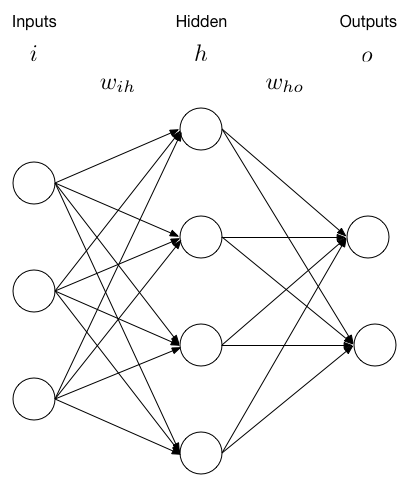
\includegraphics[width=.7\linewidth]{images/ann.png}
    \caption[An artificial neural network]{An artificial neural network with 3 input units, 4 hidden units and 2 output units. $w_{ih}$ and $w_{ho}$ are the weights for connections between respectively the input units and hidden units and between the hidden units and output units.}
    \label{fig:ann}
\end{figure}
As a non-input unit gets weighted activations from multiple units, these need to be combined to determine if the unit can be activated or not. This is done by applying a linear or non-linear function, called an activation function, to the weighted sum.
% section basics (end)

\section{Activation functions} % (fold)
\label{sec:activation_functions}
Formally, an activation function $\phi$ will compute for unit $j$ with inputs from layer $x$:
\begin{equation}
    o = \phi\big(\sum_i^n w_{ij} x_i\big)
\end{equation}
Or in vector format:
\begin{equation}
    o = \phi(\overrightarrow{w} \cdot \overrightarrow{x})
\end{equation}
From hereon we will denote the weighted sum as $z \equiv \sum_i^n w_{ij} x_i \equiv \overrightarrow{w} \cdot \overrightarrow{x}$.\\

\subsection{Perceptron} % (fold)
\label{ssub:perceptron}
A perceptron unit, defined by \cite{Rosenblatt58}, gives as output either $-1$ or $+1$ depending on the linear combination of the input and the weights:
\begin{equation}
o(\overrightarrow{x}) = \begin{cases}
+1 & \text{if $ \overrightarrow{w} \cdot \overrightarrow{x} > 0$}\\
-1 & \text{otherwise}
\end{cases}
\end{equation}
It can be seen as a hyperplane where the output is $-1$ or $+1$ depending on which side the input lies.
Using $-1$ as \texttt{false} and $+1$ as \texttt{true}, it is also possible to represent boolean functions such as \textit{AND}, \textit{OR}, \textit{NAND} and \textit{NOR}. However, some boolean functions, such as \textit{XOR} cannot be represented by a single perceptron \citep{ML}.

A schematic using the perceptron unit is shown in Figure~\ref{fig:perceptron}.\\
\begin{figure}[htb]
    \centering
    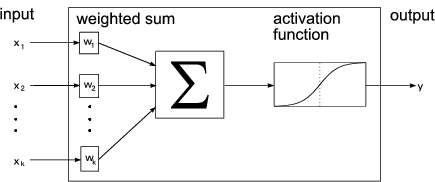
\includegraphics[width=\linewidth]{images/activation_functions/perceptron.png}
    \caption[The perceptron unit]{The perceptron unit. Source: \cite{Demant2013}.}
    \label{fig:perceptron}
\end{figure}
% subsection perceptron (end)

\subsection{Sigmoid} % (fold)
\label{ssub:sigmoid}
A disadvantage of the perceptron unit is that it is not differentiable in the whole domain (specifically at $x=0$). Why this is a problem will become clear in Section~\ref{sec:gradient_descent_and_backpropagation}.\\
To solve this problem, a sigmoid function can be used. A sigmoid function is a differentiable function that is monotonically increasing and approaches an asymptote for $x \to \pm\infty$ \citep{series/lncs/LeCunBOM12}. As a result, these can still separate the input space in 2 parts.\\
In the artificial neural networks domain, the \textit{sigmoid function} generally refers to a variation of the logistic function and is denoted by $\sigma(x)$. Its formula is:
\begin{align}
    \begin{split}
        f(z) &= \sigma(z)\\
        &= \frac{1}{1+e^{-z}}
    \end{split}
\end{align}
The behavior of this function is visualized in Figure~\ref{fig:sigmoid}.
\begin{figure}[htb]
    \centering
    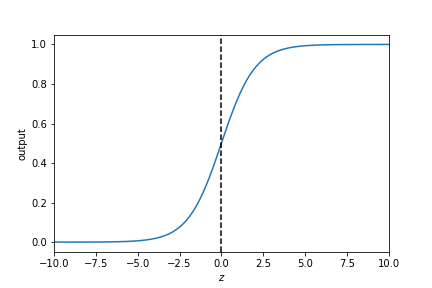
\includegraphics[width=.8\linewidth]{images/activation_functions/sigmoid.png}
    \caption[The sigmoid function]{The sigmoid function.}
    \label{fig:sigmoid}
\end{figure}
% subsection sigmoid (end)

\subsection{Hyperbolic tangent} % (fold)
\label{ssub:hyperbolic_tangent}
Another popular function and another kind of sigmoid function is the hyperbolic tangent function, also called \textit{tanh}. While the output of the sigmoid function ranges between $0$ and $+1$, here the output ranges between $-1$ and $+1$, just like the range (and the only possible values) of the perceptron.
The formula of the hyperbolic tangent function, which can also be written in terms of the sigmoid function, is:
\begin{align}
    \begin{split}
        f(z) &= tanh(z)\\
        &= 2\sigma(2z) - 1\\
        &= \frac{e^{\frac{z}{2}} - e^{-\frac{z}{2}}}{e^{\frac{z}{2}} + e^{-\frac{z}{2}}}
    \end{split}
\end{align}
This function is visualized in Figure~\ref{fig:tanh}.
\begin{figure}[htb]
    \centering
    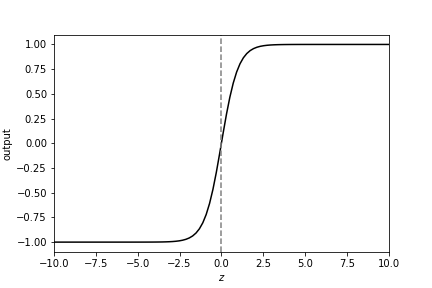
\includegraphics[width=.8\linewidth]{images/activation_functions/tanh.png}
    \caption{Hyperbolic tangent function.}
    \label{fig:tanh}
\end{figure}
% subsection hyperbolic_tangent (end)

\subsection{Rectified Linear Unit} % (fold)
\label{ssub:rectified_linear_unit}
A rectified linear unit, also called a ReLU, is another popular and more recent activation function. It was first defined by \cite{conf/icml/NairH10}. The output is the identity function if $z \ge 0$ and $0$ otherwise:
\begin{equation}
    f(z) = \begin{cases}
        z & \text{if $z \ge 0$}\\
        0 & \text{otherwise}
        \end{cases}
\end{equation}
As can be seen, this function requires less computations than the sigmoid and hyperbolic tangent function. However, the derivative for $z<0$ is always $0$. Why this can be a problem is also explained in Section~\ref{sec:gradient_descent_and_backpropagation}.\\
The ReLU function is shown in Figure~\ref{fig:relu}.
\begin{figure}[htb]
    \centering
    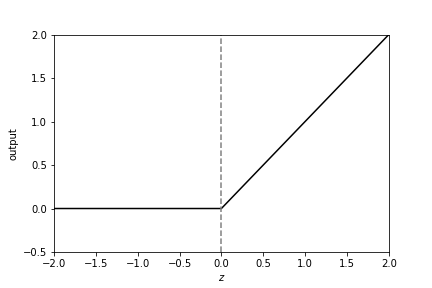
\includegraphics[width=.8\linewidth]{images/activation_functions/relu.png}
    \caption[Rectified Linear Unit function]{Rectified Linear Unit function.}
    \label{fig:relu}
\end{figure}

To solve the problem of the derivative being zero at $z<0$, the Leaky ReLU was invented \citep{maas2013rectifier}. Here, instead of the output being zero for $z<0$, the output has a small slope, defined by a constant $\alpha$:
\begin{equation}
    f(z) = \begin{cases}
        z & \text{if $z \ge 0$}\\
        \alpha z & \text{otherwise}
        \end{cases}
\end{equation}
As can be seen, the derivative of this function is always non-zero.\\
An example of a Leaky ReLU is shown in Figure~\ref{fig:lrelu}.\\
\begin{figure}[htb]
    \centering
    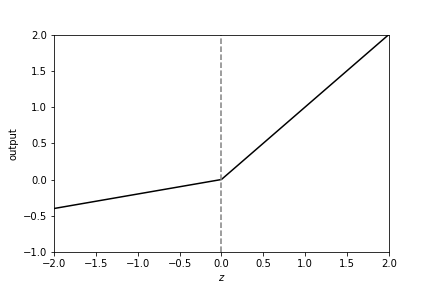
\includegraphics[width=.8\linewidth]{images/activation_functions/lrelu.png}
    \caption[Leaky ReLU function]{Leaky ReLU function with $\alpha = 0.2$.}
    \label{fig:lrelu}
\end{figure}
% subsection rectified_linear_unit (end)
% section activation_functions (end)

A variation of a Leaky ReLU, called Parametric Rectified Unit, also has a small slope for $x<0$, but with an $\alpha$ that can be learned \citep{journals/corr/HeZR015}. Other variants use a random slope for values below zero \citep{journals/corr/XuWCL15}, add noise a ReLU \citep{conf/icml/NairH10} or use an exponential function for values below zero \citep{journals/corr/ClevertUH15}:
\begin{equation}
    f(z) = \begin{cases}
        z & \text{if $z \ge 0$}\\
        \alpha (e^z-1) & \text{otherwise}
        \end{cases}
\end{equation}

\todo{Add softmax (used in my network)}


\section{Gradient descent and backpropagation} % (fold)
\label{sec:gradient_descent_and_backpropagation}
%Also something about linearly separable?
%Why no algebraic solution?
If we choose the weights of our network correctly, we might succeed in approximating a function.
However, it is not always possible to separate the input space and have the right with our artificial neural network.
In that case, we might want the best solution, e.g. one that has the least amount of errors in producing outputs w.r.t. the correct outputs, also called the target outputs. Furthermore, choosing the weights manually can be a tedious process.\\
For these reasons, we use an algorithm called called backpropagation, which uses a variation of gradient descent. We will first discuss gradient descent as this provides the basis of the backpropagation algorithm.

\subsection{Gradient descent} % (fold)
\label{ssub:gradient_descent}
In gradient descent, we search in the weight vector space, also called hypothesis space, to find weights that can approximate a function as best as possible. A tuple containing the input and output of the target function is called a training example.

To be able to update weights, we first need to know how wrong our outputs were relative to those of our training examples.
This is called the training error and depends on the learning algorithm (in our case an artificial neural network), its parameters and the training examples. However, here we assume that the learning algorithm and the training examples are fixed while learning.
A common measure for the training error, the mean squared error (MSE), is defined as:
\begin{equation}
    E(\overrightarrow{w}) \equiv \frac{1}{N} \sum_{i=0}^N (y_i - f(x_i;\overrightarrow{w}))^2
\end{equation}
Where $N$ is the number of training examples, $x_i$ is the input of a training example, $y_i$ is the target output of the training example and $f$ is our learning algorithm, which depends on the weight vector $\overrightarrow{w}$.\\

Because we now know how the training error and the weight vector are related, we can compute the derivative of the training error $E$ with respect to each component of $\overrightarrow{w}$. This called the gradient and is denoted as $\nabla E(\overrightarrow{w})$:
\begin{equation}
    \nabla E(\overrightarrow{w}) \equiv \left [ \frac{\partial E}{\partial w_0}, \frac{\partial E}{\partial w_1}, \dots, \frac{\partial E}{\partial w_n} \right ]
\end{equation}
Where $n$ is the number of components in $\overrightarrow{w}$. Note that $\nabla E(\overrightarrow{w})$ is also a vector. It defines how to change the weight components in order to get the steepest increase in the training error $E$. Thus, if we negate the gradient, we get the steepest decrease in $E$. We can then update the weight vector as such:
\begin{equation}
    \overrightarrow{w} \gets \overrightarrow{w} - \eta \nabla E(\overrightarrow{w})
\end{equation}
Where $\eta$ is a positive value called the learning rate, which influences how big the changes to the weight vector are.\\

The goal is to set the weights to such values so that the error is minimized. This is called a global minimum. No other combinations of weight values can lead to a lower error an those of the global minima.\\
However, it is possible that, given a combination of weight values, any change in those values does not influence the error, in which case the gradient for every weight component is $0$. Thus, with the current algorithm, there is no incentive to change the weights. This is called a local minimum. Although the algorithm cannot "see" immediate improvements, it is possible that another combination of weight values leads to a lower error. This is analogous to being in a valley in the mountains, where the valley after a mountain (and thus not visible) may lie lower. This is also visualized in Figure~\ref{fig:error_surface}.\\
\begin{figure}[htb]
    \centering
    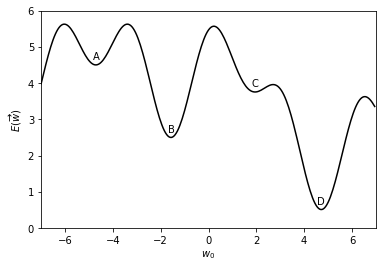
\includegraphics[width=\linewidth]{images/error_surface.png}
    \caption[An example of an error surface]{An example of an error surface using only one weight $w_0$. \textit{A}, \textit{B} and \textit{C} are local minima, while \textit{D} is the global minimum.}
    \label{fig:error_surface}
\end{figure}
Local minima might seem like a problem for neural networks, but in practice they rarely are, according to theoretical and empirical results \citep{choromanska2015loss}.
Instead, there are more saddle points. Here, the gradient is zero and the error goes up when some weights are changed and goes down for others. Generally a lot of such points are present, but they all have the same value for the objective function (i.e. the error function).\\

A small value of $\eta$ leads to slow convergence, while a high value can cause the algorithm to overstep a local minimum. Because of this, the some algorithms gradually decrease the learning rate as the number of weight updates grows.\\
For a single weight component, we get:
\begin{equation}
    \label{eq:weightcomponentupdate}
    w_i \gets w_i - \eta \frac{\delta E}{\delta w_i}
\end{equation}

Of course, in order to update the weights, we first need to calculate the derivate of $E$ w.r.t. each component $w_i$. As an example, we show the derivative when using a simple linear unit, which defined as:
\begin{equation}
    f(\overrightarrow{x};\overrightarrow{w}) = \overrightarrow{x} \cdot \overrightarrow{w}
\end{equation}
We then get the following derivation:
\begin{align}
    \label{eq:gradderiv}
    \begin{split}
        \frac{\delta E}{\delta w_i} &= \frac{\delta}{\delta w_i} \frac{1}{N} \sum_{j=0}^N (y_j - o_j)^2\\
        &= \frac{1}{N} \sum_{j=0}^N \frac{\delta}{\delta w_i} (y_j - o_j)^2\\
        &= \frac{1}{N} \sum_{j=0}^N 2 (y_j - o_j) \frac{\delta}{\delta w_i} (y_j - o_j)\\
        &= \frac{2}{N} \sum_{j=0}^N (y_j - o_j) \frac{\delta}{\delta w_i} (y_i - \overrightarrow{x_i} \cdot \overrightarrow{w})\\
        &= \frac{2}{N} \sum_{j=0}^N (y_j - o_j)(-x_{ij})
    \end{split}
\end{align}
Where $x_{ij}$ is the $i$'th input component of training example $j$ and $o_j \equiv f(x_j; \overrightarrow{w})$. Instead of just using a linear unit, the function $f$ can of course be more complex and use for example on of the activation functions from Section~\ref{sec:activation_functions}. However, we can now see that we cannot use the perceptron because it is not differentiable.\\

Using the resulting formula of Equation~\ref{eq:gradderiv} along with Equation~\ref{eq:weightcomponentupdate}, we can also define how to update each component of the weight vector:
\begin{equation}
    w_i \gets w_i + \eta \frac{2}{N} \sum_{j=0}^N (y_j - o_j)x_{ij}
\end{equation}
As we can see, for each weight vector, we need to apply the model to the input of each training example. For this reason, this version of gradient descent is also often called \textit{batch gradient descent}. Of course, the outputs only need to be computed once per weight vector update as they do not depend on which specific weight vector component that we are updating.\\

Still, each time using every training example for the weight vector update can lead to slow convergence to a local minimum. Furthermore, in case of multiple local minima in the error surface, it is possible that the gradient descent algorithm does not stop at the global minimum \citep{ML}.
% subsection gradient_descent (end)

\subsection{Stochastic gradient descent} % (fold)
\label{ssub:stochastic_gradient_descent}
A popular variation of batch gradient descent that tries to solve the previously mentioned issues is \textit{stochastic gradient descent}. Instead of summing using all training examples, we do a weight update using only one training example. To do this, we first use a different error function for each example $j$:
\begin{equation}
    E_j(\overrightarrow{w}) = (y_j - o_j)^2
\end{equation}
The update for a single weight vector component when using a linear unit is then:
\begin{equation}
    w_i \gets w_i + 2 \eta(y_j- o_j)x_{ij}
\end{equation}
The idea here is that these weight updates, when having iterated over all the training examples, will be a decent approximation relative to using our original error function. Note that the update using one training example affects the error of the next training example.\\

By making the learning rate small enough, usually smaller than with batch gradient descent, it is possible to approximate true gradient descent arbitrarily closely \citep{ML}.
It is also computationally cheaper because each time we only handle one training example.
Additionally, stochastic gradient descent can sometimes avoid being stuck in local minima because it uses various $\nabla E_j(\overrightarrow{w})$ instead of just $\nabla E(\overrightarrow{w})$ to move in the hypothesis space.
% subsection stochastic_gradient_descent (end)

\subsection{Backpropagation} % (fold)
\label{ssub:backpropagation}
The backpropagation algorithm uses gradient descent and can learn weights of a multilayer network with possibly multiple units in each layer \citep{rumelhart1986learning}.

We say that, for multilayer networks, $L>2$, with $L$ the number of layers in the network. This means that there are other (hidden) layers besides the input and output layer. Such a network was already depicted in Figure~\ref{fig:ann}.

As multiple output units are also possible, we need a new training error measure that sums over all of the output units of the network:
\begin{equation}
    E(\overrightarrow{w}) \equiv \frac{1}{N} \sum_{i=0}^N \sum_{k \in outputs} (y_{ki} - o_{ki})^2
\end{equation}
Where $outputs$ are the output units of the network and $y_{ki}$ and $o_{ki}$ is the value of the $k$'th output unit of respectively the $i$'th training example and network output.\\

The difference with calculating the weight changes in artificial neural networks with more than 2 layers is that, starting from the second non-input layer, the input to a unit comes, besides the weights, from other units of which the value itself is also calculated.
Thus, units in some layers can depend on units in multiple previous layers. This must also be taken into account when calculating the gradient for the output of those units.
To do this, we can use the chain rule for the gradient of a single weight component:
\begin{align}
    \frac{\partial E_d}{\partial w_{ji}} &= \frac{\partial E_d}{\partial net_j} \frac{\partial net_j}{\partial w_{ji}}\\
    &= \frac{\partial E_d}{\partial net_j} x_{ji}
\end{align}
Where $E_d$ is the error for a training example $d$, $x_{ji}$ is the $i$'th input to unit $j$, $w_{ji}$ is the weight associated with this input and $net_j = \sum_i w_{ji} x_{ji}$. The further derivation for all the weights of the network is described in \cite[Chapter~4]{ML}. For an artificial neural network with 1 hidden layer, we get the pseudo-code shown in Algorithm~\ref{algo:backpropagation}.\\
\begin{algorithm}[htb]
\DontPrintSemicolon
\KwIn{training\_examples, neural\_network, $\eta$}
\emph{// Assume a network with $n_{in}$ input units $n_{hidden}$ hidden units and $n_{out}$ output units.}\\
\emph{// Assume (randomly) instantiated weights.}\\
\Repeat{a termination condition is met}{
    \For{$(\overrightarrow{x},\overrightarrow{y})$ in training\_examples}{
        Propagate $\overrightarrow{x}$ through the network and receive values for all the output units: $o_u$ with $u$ an output unit of the network\\
        \For{each network output unit $k$}{
            Calculate its error term:\\
            $\delta_k \gets o_k(1-o_k)(y_k-o_k)$
        }
        \For{each hidden unit $h$}{
            Calculate its error term:\\
            $\delta_h \gets o_h(1-o_h) \sum_{k \in outputs} w_{kh}\delta_k$
        }
        \For{each network weight $w_{ji}$}{
            Do an update:\\
            $w_{ji} \gets w_{ji} + \Delta w_{ji}$\\
            where\\
            $\Delta w_{ji} = \eta \delta_j x_{ji}$ \label{algo:backpropagation:deltaweight}
        }
    }
}
\caption[Backpropagation]{Backpropagation algorithm. For simplicity, the squared error ($E_j(\overrightarrow{w}) = \frac{1}{2} (y_j - o_j)^2$ for training example $j$) was used. Source: \cite[Chapter~4]{ML}.}
\label{algo:backpropagation}
\end{algorithm}
% subsection backpropagation (end)

\subsection{Extensions and improvements} % (fold)
\label{ssub:extensions_and_improvements}
\paragraph{Different loss functions} % (fold)
\label{par:loss_functions}
Besides just the difference between the output of the network and the expected output, additional penalties can be added to indirectly influence the values of the weights.
Here, we typically use the term loss function instead of an error function. This loss function can contain the error as we already described, along with other functions (typically also called loss functions).\\

A popular loss function is called the $L_1$ norm (also called Lasso) \citep{tibshirani1996regression}. For each weight $w$, we add the value $\lambda \vert w \vert$ to the loss. The $L_1$ norm is then defined as such:
\begin{equation}
    L_1(\overrightarrow{w}) = \lambda \sum_{i=1}^k \vert w_i \vert
\end{equation}
Where $k$ is the number of weights of the network and $\lambda$ is a parameter determining the regularization strength.
As the loss function, we then get:
\begin{equation}
    L(\overrightarrow{w}) = E(\overrightarrow{w}) + L_1(\overrightarrow{w})
\end{equation}
This norm has the property of leading to sparse weight vectors \citep{journals/ftml/BachJMO12}. This means that a lot of weights are zero or close to zero and the focus is on finding a subset of the must important units.
%neurons with L1 regularization end up using only a sparse subset of their most important inputs and become nearly invariant to the “noisy” inputs

Instead of using the absolute value, the $L_2$ norm sums over squared weights. It has the following form:
\begin{equation}
    L_2(\overrightarrow{w}) = \frac{1}{2} \sum_{i=1}^k w_i^2
\end{equation}
The fraction $\frac{1}{2}$ is often used such that the derivative is $\lambda w$ instead of $2 \lambda w$. The $L_2$ loss focuses more on penalizing high weights. It leads to diffusion of the weights and can indirectly force the network to use all the units of the network to form the correct output.
% notice that during gradient descent parameter update, using the L2 regularization ultimately means that every weight is decayed linearly: W += -lambda * W towards zero.

The $L_1$ and $L_2$ can also be combined, called \textit{elastic net regularization} \citep{hastie2012ElasticNet}:
\begin{align}
    L_E (\overrightarrow{w}) &= L_1(\overrightarrow{w}) + L_2(\overrightarrow{w})\\
    &= \sum_{i=1}^k \lambda_1 \vert w_i \vert + \lambda_2 w_i^2
\end{align}

% paragraph loss_functions (end)

\paragraph{Different weight updates} % (fold)
\label{par:different_weight_updates}
Here we discuss methods that, given an error function, update the weights in different ways.\\

One of the most common extensions to backpropagation is to add a fraction of the previous weight update to the new weight update. This extension is called \textit{momentum}.\\
To apply this, we change the equation on line~\ref{algo:backpropagation:deltaweight} of Algorithm \ref{algo:backpropagation} to the following:
\begin{equation}
    \Delta w_{ji}(t) = \eta \delta_j x_{ji} + \alpha \Delta w_{ji}(t-1)
\end{equation}
Where $\Delta w_{ji}(t)$ is a weight update executed at iteration $t$ and $\alpha$, with $0 \le \alpha < 1$, determines how much of the previous weight update we want to carry to the new one. When $\alpha = 0$, we get again the regular weight update.

Thanks to momentum, it is possible to get past regions where the gradient is zero and the weights would not change without momentum.
This is analogous to a ball rolling down a surface but keeps rolling a bit on a flat surface afterwards. In the real world, an object in motion will stay in motion, unless there is a force applied to it.
Here, that force is the gradient. It is also possible to get past small local minima and it can speed up learning when the gradient does not change. Again, this is analogous to a ball that goes downhill and keeps gaining speed.\\

The weight update of Root Mean Square Propagation (RMSProp) is quite different from stochastic gradient descent and only uses the sign of the gradient to update the weights \citep{Tieleman2012LectureMagnitude.}.
This allows us to escape from plateaus more quickly. Furthermore, the learning rate can be different for each weight.
For example, we can multiply the learning rate of a certain weight by a factor greater than one if its last 2 gradients agreed on the sign, and multiply the learning rate by a value less than $1$ otherwise.
This means that, when the gradients agree on the direction, we give them more influence. If they are not consistent and disagree in subsequent steps, we decrease the influence. We can also put a limit on the learning rate as to not let it grow to excessively low or high amounts.

However, by just using an adaptive learning rate, we can have the problem of weights themselves growing too high in unwanted situations. For example, when a gradient is for 9 subsequent steps a small positive amount (e.g. $0.1$) and once a large negative amount (e.g. $-0.9$), we don't want to change the weights a lot because they balance each other out.
Using the current algorithm however, the learning rate and as a result the weights would become too high because we only look at the signs and not the magnitude of the gradients.\\
Notice that, right now, we are dividing the gradient by its absolute value in order to just get $+1$ or $-1$ depending on the sign. It is however better to divide each weight by a moving average of the squared weight using the gradients of the past steps:
\begin{subequations}
\label{eq:rmsprop}
\begin{align}
MeanSquare(w, t) &= \gamma \cdot MeanSquare(w, t-1) + (1 - \gamma) \cdot \left (\frac{\partial E}{\partial w(t)} \right )^2 \\
w(t+1) &= w(t) - \frac{\alpha}{\sqrt{MeanSquare(w,t)}}\frac{\partial E}{\partial w(t)} \label{eq:rmsprop:weightupdate}
\end{align}
\end{subequations}
Where $w(t)$ is a weight at time step $t$, $\frac{\partial E}{\partial w(t)}$ is its gradient, $\alpha$ is the learning rate and $w_{t+1}$ is the new weight value. The past squared gradients are decayed by a value $\gamma$. Usually $\gamma=0.9$. It is also possible to add a small number $\epsilon$ (e.g. $\epsilon = 10^{-8}$) to the denominator in Equation~\ref{eq:rmsprop:weightupdate} to avoid division by zero.\\

Adaptive Moment Estimation (Adam) \citep{DBLP:journals/corr/KingmaB14} also uses an adaptive learning rate for each weight and an exponentially decaying average of previous squared gradients (also called the second moment). In addition, an exponentially decaying average of past gradients (also called the first moment) is also stored:
\begin{subequations}
\label{eq:adam:means}
\begin{align}
    Mean(w,t) &= \beta_1 \cdot Mean(w,t-1) + (1-\beta_1)\cdot \frac{\partial E}{\partial w(t)}\\
    MeanSquare(w, t) &= \gamma \cdot MeanSquare(w, t-1) + (1 - \gamma) \cdot \left (\frac{\partial E}{\partial w(t)} \right )^2
\end{align}
\end{subequations}
The authors of this method observed that the two previous equations are biased towards zero, which results in high weight updates. To alleviate this problem, the use bias-corrected values:
\begin{subequations}
\label{eq:adam:means:corrected}
\begin{align}
    \widehat{Mean(w,t)} &= \frac{Mean(w,t)}{1-\beta_1^t}\\
    \widehat{MeanSquare(w,t)} &= \frac{MeanSquare(w,t)}{1-\beta_2^t}
\end{align}
\end{subequations}
The weight update then becomes:
\begin{equation}
    w(t+1) = w(t) - \frac{\alpha}{\sqrt{MeanSquare(w,t)} + \epsilon} Mean(w,t)
\end{equation}
% paragraph different_weight_updates (end)
% subsection extensions_and_improvements (end)
% section gradient_descent_and_backpropagation (end)

% Inspired by biology

% section artificial_neural_networks (end)

\chapter{Reinforcement learning}
\label{cha:reinforcement_learning}
%\cite{Sutton1998ReinforcementIntroduction.}.
In reinforcement learning, one tries to find which action to take in a certain state of the environment in order to maximize a possibly delayed numerical reward.\\
For chapters \ref{sub:rl:basics} to \ref{sec:rl:bootstrapping} and \ref{sub:rl:gfa}, we will closely follow the explanation by \cite{Sutton1998ReinforcementIntroduction}.

\section{Basics}
\label{sub:rl:basics}
Reinforcement learning problems can be formulated in the form of a Markov Decision Process (MDP). This is four-tuple $(\mathcal{S}, \mathcal{A}, \mathcal{P}, \mathcal{R})$. $\mathcal{S}$ is the state space and contains all the possible states of the environment. The action space, $\mathcal{A}$, denotes all the possible actions that the agent can take in the environment. $\mathcal{P}: \mathcal{S} \times \mathcal{A} \to \mathcal{S}$ is the transition function and defines the probabilities for being in next state given a state and an action. $\mathcal{R}: \mathcal{S} \times \mathcal{A} \to \mathcal{R}$ gives probabilities for rewards when taking an action in a certain state. A transition is then a tuple of a state, an action taken at that state, the received reward by taking that action (determined using $\mathcal{R}$) and the next state (determined using $\mathcal{P}$): $(s_t,a_t,r_t,s_{t+1})$. A sequence of transitions is called a trajectory.

A reinforcement learning algorithm does not know on beforehand which actions are optimal. As such, this must be discovered by trial-and-error. Subsequently, it can change its policy to increase the achieved rewards. This policy, denoted by $\pi$, defines for each state and action a probability $\pi(s,a)$, which denotes the probability of taking action $a$ when in state $s$: $\pi_t(s,a) = P(a_t = a \vert s_t = s)$. Note that exactly one action has to be taken in a state and that the action probabilities for one state sum to $1$: $\sum_{a\in \mathcal{A}}\pi_t(s,a)=1$.\\
Because feedback in the form of numerical rewards may not be immediate, a reinforcement learning algorithm must be able to backtrack which actions in certain situation lead to the reward that the reinforcement learning algorithm received.\\

Reinforcement learning algorithms often use a state-value function $V(s)$. This function says how good it is to be in a certain state $s$ by stating the expected return in the future starting from state $s$, where the return is the discounted rewards. This expected value when starting in state $s$ and following a specific policy $\pi$ is denoted as $V^\pi(s)$:
\begin{equation}
\label{eq:vpolicy}
V^\pi(s) = \ex_\pi\{R_t \vert s_t=s\}=\ex_\pi\big \{ \sum_{k=0}^{\infty}\gamma^k r_{t+k+1} \vert s_t=s\big \}
\end{equation}
Where $\gamma$ is a discount applied over time to past rewards. The optimal policy $\pi$ is the one that leads to the highest $V^\pi(s)$ for all $s \in \mathcal{S}$. The resulting state-value function is $V^*(s) = \max_\pi V^\pi(s)$ for all $s \in \mathcal{S}$.

% Like for states, it is also possible to use the value of an action $Q_t(a)$ at time step $t$. Which can be calculated by averaging the rewards obtained by applying action $a$ to time step $t$:
% \begin{equation}
% Q_t(a) = \frac{r_1 + r_2 + \dots + r_{k_a}}{k_a}
% \end{equation}

It is also possible to define a value for taking an action in a certain state, which is the action-value function $Q(s,a)$. $Q^\pi(s,a)$ is the expected return after taking action $a$ in state $s$:
\begin{equation}
Q^\pi(s,a) = \ex_\pi\{R_t|s_t=s,a_t=a\}=\ex_\pi\big \{ \sum_{k=0}^{\infty}\gamma^k r_{t+k+1} | s_t=s,a_t=a\big \}
\end{equation}
Similarly as with $V^*(s)$, $Q^*(s,a)$ is the action-value function we have when applying the optimal policy.\\
Actions can be selected by for example $\epsilon$-greedy or softmax. In $\epsilon$-greedy action selection, the action with the highest $Q(s,a)$ is selected with probability $1-\epsilon$ and a random action otherwise.\\
Softmax chooses an action $a$ when in state $s$ with the following probability:
\begin{equation}
p(s,a) = \frac{e^{Q(s,a)/\tau}}{\sum_{b=1}^n e^{Q(s,b)/\tau}}
\end{equation}
Where $\tau$ is called the temperature and controls the balance between exploration and exploitation. For low values, the best actions are highly probable. For $\tau \to 1$, the probability distribution becomes uniform.\\

%Chapter 4
\section{Dynamic programming}
\label{sub:rldp}
In Dynamic programming, the whole model of the problem is known. A such, we have the complete probability distribution of all the possible transitions. For example, to evaluate a policy $\pi$:
\begin{align}
\begin{split}
V^{\pi}(s) &= \ex_{\pi} \{r_{t+1} + \gamma r_{t+2} + \gamma^2r_{t+3}+\dots \mid s_t=s\}\\
&= \ex_{\pi} \{r_{t+1} + \gamma V^{\pi}(s_{t+1}) \mid s_t=s\}\\
&= \sum_a \pi(s,a) \sum_{s'} \mathcal{P}^a_{ss'} [\mathcal{R}^a_{ss'} + \gamma V^{\pi}(s')]
\end{split}
\end{align}
Here, $\pi(s,a)$ is the probability of taking action $a$ in state $s$. This $V^{\pi}(s)$ can be computed using iterative updates for every $s$:
\begin{align}
\begin{split}
V_{k+1}(s) &= \ex_{\pi}\{r_{t+1} + \gamma V_k(s_{t+1}) \vert s_t=s\}\\
&= \sum_a \pi(s,a) \sum_{s'}\mathcal{P}^a_{ss'} [\mathcal{R}^a_{ss'} + \gamma V_k(s')]
\end{split}
\end{align}
This iteration stops when this state-value function has converged. As can be seen, every possible next states is used in the computation instead of just a sample. Because of this, this kind of updates is called a full backup.
Note that we use an estimate of the value function to update the estimate itself. This is called bootstrapping.\\
The optimal state-value function $V^*(s)$ and state-action-value function $Q^*(s,a)$ can be calculated using the following formulas:
\begin{gather}
\begin{split}
V^{*}(s) &= \max_a E\{r_{t+1} + \gamma V^{*}(s_{t+1}) \vert s_t = s, a_t = a\}\\
&= \max_a \sum_{s'} \mathcal{P}^a_{ss'} [\mathcal{R}^a_{ss'}+\gamma V^{*}(s')]
\end{split}\\
\begin{split}
Q^{*}(s,a) &= E\{r_{t+1} + \gamma \max_{a'} Q^{*}(s_{t+1},a') \vert s_t=s, a_t=a\}\\
&= \sum_{s'} \mathcal{P}^a_{ss'} [\mathcal{R}^a_{ss'}+\gamma \max_{a'} Q^{*}(s',a')]
\end{split}
\end{gather}

\section{Monte Carlo and Temporal-Difference}
\label{sub:rl_mctd}
Unlike dynamic programming, model-free methods don't require complete knowledge of the environment. Instead, only sample transitions are needed. This way, 2 problems with dynamic programming can be solved. First, the model may be large, which makes it infeasible to use for computing for example an optimal policy. Second, in real world problems, a complete model of the problem may not be available. It may for example be unknown what is the probability of ending in a certain state when taking a certain action from a start state.\\
Monte Carlo methods collect sample returns and average them in order to approximate a value function. The incremental implementation for approximating $V$ is as follows:
\begin{equation}
V(s_t) \leftarrow V(s_t) + \alpha\big[R_t - V(s_t)\big]
\end{equation}
Where $R_t$ is the actual return of an action and $\alpha$ is a constant step-size parameter. As was shown in equation \ref{eq:vpolicy}, to compute $R_t$ we need all the future rewards until the end of the episode.\\
Temporal-Difference (TD) learning tries to solve this by bootstrapping techniques like in dynamic programming. To do this, in the update we replace the full return using the observed reward and the estimate of the value of the next state. This is known as TD(0):
\begin{equation}
V(s_t) \leftarrow V(s_t) + \alpha\big[r_{t+1}+\gamma V(s_{t+1}) - V(s_t)\big]
\end{equation}
These estimates can then be used for acting in an environment.\\
Sarsa uses TD estimates for on-policy control. Because it is on-policy, we must estimate the action-value function $Q^\pi(s,a)$ for the current behavior policy $\pi$ and for all states $s$ and actions $a$. We consider transitions from state-action pair to state-action pair instead of transitions from state to state. The update is as follows:
\begin{equation}
Q(s_t,a_t) \leftarrow Q(s_t,a_t) + \alpha \big[ r_{t+1} + \gamma Q(s_{t+1},a_{t+1}) - Q(s_t,a_t) \big]
\end{equation}
We can then choose the action with the highest $Q^\pi(s_t,a_t)$, using $\epsilon$-greedy etc.
%The Gamma parameter has a range of 0 to 1 (0 <= Gamma > 1).  If Gamma is closer to zero, the agent will tend to consider only immediate rewards.  If Gamma is closer to one, the agent will consider future rewards with greater weight, willing to delay the reward.
Another control method called Q-learning also uses TD estimates but doesn't use the policy that is followed to estimate $Q^*$. This is called an off-policy algorithm. Here, we do a backup using the action that has the highest $Q$ value at the next state:
\begin{equation}
Q(s_t,a_t) \leftarrow Q(s_t,a_t) + \alpha \big[ r_{t+1} + \gamma \max_{a} Q(s_{t+1}, a) - Q(s_t,a_t) \big]
\end{equation}
Note that the policy still can influence which state-action pairs are visited and updated. To guarantee finding the optimal behavior, it is required that all pairs continue to be updated.\\

%Chapter 7
\section{Eligibility traces}
\label{sub:rl_et}
Eligibility traces are used in order to only influence eligible states or actions when a certain action is taken.\\
%$n$-Step TD prediction
Monte Carlo methods perform a backup for each state based on the entire sequence of observed rewards from that state until the end of the episode. The backup of more simple methods is only based on the next reward of a state, using the state value one step later as a proxy for the remaining rewards. An intermediate method would perform a backup based on an intermediate number of rewards. Then, we use the rewards of the intermediate steps and the estimated value of the last state. A visualization can be seen in Figure \ref{fig:nStepTD}.
\begin{figure}[htb]
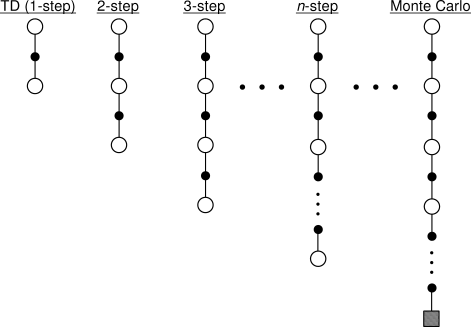
\includegraphics[width=\linewidth]{images/nStepTD.png}
\caption[$n$-step returns]{Returns each based on a different amount of rewards and by using the state value as a proxy afterwards. This is not needed for Monte Carlo methods as they use all the future rewards. Source: \cite{Sutton1998ReinforcementIntroduction}.}
\label{fig:nStepTD}
\end{figure}
The $n$-step target can be formulated as:
\begin{equation}
R_t^{(n)} = r_{t+1} + \gamma r_{t+2} + \dots + \gamma^{n-1}r_{t+n} + \gamma^n V_t(s_{t+n})
\end{equation}
There, we treat the terminal state as a state that always transitions to itself with zero reward. This way of treating an episodic task the same as a continuing task doesn't influence the result, even if we discount the returns. As such, all $n$-step returns that last up to or past termination have the same value as the complete return.\\
The increment to $V_t(s_t)$ is then defined by:
\begin{equation}
\Delta V_t(s_t) = \alpha \big[ R_t^{(n)} - V_t(s_t) \big]
\end{equation}
In on-line updating, the updates are done during the episode, as soon as a $\Delta V_t(s_t)$ is computed. In off-line updating, these increments are set aside and applied after the episode is done.\\
$n$-step TD methods are rarely used because they are inconvenient to implement. To compute $n$-step returns, you have to wait $n$ steps to observe the resultant rewards and states.\\

We can also take the weighted average of $n$-step return. This is called the forward view or theoretical view. The requirement is that the weights sum to 1. TD($\lambda$) is a particular way of doing this. The $\lambda$-return is defined by
\begin{equation}
R^\lambda_t = (1-\lambda) \sum_{n=1}^{\infty} \lambda^{n-1} R_t^{(n)}
\end{equation}
After a terminal state has been reached, all subsequent $n$-step returns are equal to $R_t$, so the $(1-\lambda)$ isn't applied. When $\lambda=1$, we will only have the conventional return $R_t$. The increment, $\Delta V_t(s_t)$, is:
\begin{equation}
\Delta V_t(s_t) = \alpha \big[ R_t^{\lambda} - V_t(s_t) \big]
\end{equation}
In this forward view, we look for each state visited forward in time to all the future rewards and decide how best to combine them. After looking forward from and updating one state, we move to the next and don't work with that state anymore. Future states, however, are viewed and processed repeatedly. This way of thinking is visualized in Figure \ref{fig:TDForwardView}.
\begin{figure}[htb]
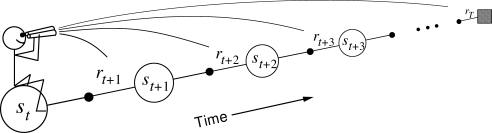
\includegraphics[width=\linewidth]{images/TDForwardView.png}
\caption[TD forward view]{The forward view, where each state value is updated by looking forward to the states and their rewards that follow. Source: \cite{Sutton1998ReinforcementIntroduction}.}
\label{fig:TDForwardView}
\end{figure}

The backward view can be seen as a practical version of the forward view, as it achieves the same but is easier to implement.
Here we have an additional memory variable associated with each state, the eligibility trace, denoted $e_t(s) \in \rm I\!R^+$. On each step, they are decayed by $\gamma \lambda$, and the eligibility trace for the one state visited on the step is incremented by 1. The increment $\Delta V_t(s_t)$ is then defined as such:
\begin{subequations}
\label{eq:backview}
\begin{align}
\delta_t &= r_{t+1} + \gamma V_t(s_{t+1}) - V_t(s_t) \label{eq:backview1} \\
\Delta V_t(s) &= \alpha \delta_t e_t(s), \qquad \text{for all} \quad s \in S \label{eq:backview2}
\end{align}
\end{subequations}
Here we work backwards and update backward to each prior state according to the state's eligibility trace at that time. This is visualized in Figure \ref{fig:TDBackwardView}.
\begin{figure}[htb]
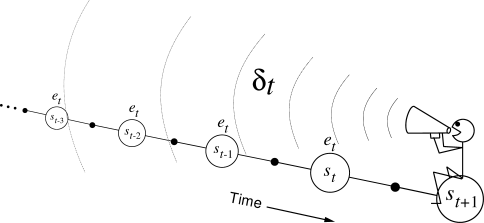
\includegraphics[width=\linewidth]{images/TDBackwardView.png}
\caption[TD backward view]{The backward view, where the value of visited states are updated based on their eligibility values. Source: \cite{Sutton1998ReinforcementIntroduction}.}
\label{fig:TDBackwardView}
\end{figure}
If we set $\lambda = 0$, then we only update the trace for $s_t$, thus getting TD(0). For larger values, with $\lambda < 1$, more of the preceding states are changed. The more distant states are changed by a smaller amount because the eligibility trace is smaller. This way, they are blamed less for the TD error.\\
If $\lambda = 1$ the credit given to earlier states falls only by $\gamma$ per step. If $\lambda = 1$ and $\gamma = 1$, then there is no decay at all and we achieve the Monte Carlo method for an undiscounted episodic task. This is known as TD(1). This TD(1) is more general however because it cannot only be applied to episodic tasks, but also to discounted continuing tasks. It can also be performed incrementally and on-line, while Monte Carlo methods have to wait until the episode is over. If the Monte Carlo control method does something bad, its behavior cannot change during the same episode, while on-line TD(1) can (using $n$-step).\\
Both methods achieve the same weight update.\\

To combine TD($\lambda$) and Sarsa, called Sarsa($\lambda$), we need eligibility traces for each state-action pair: $e_t(s,a)$. As such, we do updates like this:
\begin{equation}
Q_{t+1}(s,a) = Q_t(s,a) + \alpha \delta_t e_t(s,a), \qquad \text{for all} \quad s,a
\end{equation}
where
\begin{equation}
\delta_t = r_{t+1} + \gamma Q_t(s_{t+1},a_{t+1}) - Q_t(s_t,a_t)
\end{equation}
and
\begin{equation}
e_t(s,a) = \begin{cases}
    \gamma \lambda e_{t-1}(s,a) + 1 & \text{if $s=s_t$ and $a=a_t$;} \\
    \gamma \lambda e_{t-1}(s,a) & \text{otherwise}.
\end{cases}
\qquad \text{for all $s,a$}
\end{equation}
The resulting algorithm can be seen in Algorithm~\ref{algo:sarsalambda}:\\
\begin{algorithm}[htb]
\DontPrintSemicolon
Initialize $Q(s,a)$ arbitrarily\;
$e(s,a) \gets 0$ for all $s,a$\;
\For{each episode} {
    Initialize s,a\;
    \Repeat{$s$ is terminal} {
        Take action $a$, observe reward $r$ and new state $s'$\;
        Choose action $a'$ from $s'$ with action selection policy using $Q$\;
        $\delta = r + \gamma Q(s',a') - Q_t(s,a)$\;
        $e(s,a) \gets e(s,a) + 1$\;
        \For{all $s,a$} {
            $Q(s,a) \gets Q(s,a) + \alpha \delta e(s,a)$\;
            $e(s,a) \gets \gamma \lambda e(s,a)$\;
        }
        $s \gets s'$; $a \gets a'$\;
    }
}
\caption[Sarsa($\lambda$)]{Sarsa($\lambda$). Source: \cite{Sutton1998ReinforcementIntroduction}}
\label{algo:sarsalambda}
\end{algorithm}
Two methods exist to combine TD($\lambda$) and Q-learning and thus getting Q($\lambda$): There exists 2 different methods: Watkins' Q($\lambda$) and Peng's Q($\lambda$).\\
Here, we must cut off the look ahead until the first exploratory action instead of the episode's end. This is done because this exploratory action doesn't have any relationship with the greedy policy. Recall that Q-learning is an off-policy method and the policy learned about is not necessarily the same as the one used to select actions. As such, it can learn about the greedy policy while following a policy involving exploratory (suboptimal) actions.

For Watkins' Q($\lambda$), if $a_{t+n}$ is the first exploratory action, the longest backup is toward:
\begin{equation}
r_{t+1} + \gamma r_{t+2} + \dots + \gamma^{n-1} r_{t+n} + \gamma^n \max_a Q_t(s_{t+n},a)
\end{equation}
Where we assume off-line updating.\\
In the backward view, we update the eligibility traces just like in Sarsa, with the only exception that we don't use the eligibility trace of the previous time step when a suboptimal (exploratory) action is taken. We get the following result:
\begin{equation}
e_t(s,a) = I_{s s_t} * I_{a a_t} + \begin{cases}
    \gamma \lambda e_{t-1}(s,a) & \text{if $Q_{t-1}(s_t,a_t) = \max_a Q_{t-1}(s_t,a)$;} \\
    0 & \text{otherwise}
\end{cases}
\end{equation}
Where $I_{xy}$ is an identity indicator function, equal to $1$ if $x=y$ and $0$ otherwise. The Q update is defined by:
\begin{equation}
Q_{t+1}(s,a) = Q_t(s,a) + \alpha \delta_t e_t(s,a)
\end{equation}
Where
\begin{equation}
\delta_t = r_{t+1} + \gamma \max_{a'} Q_t(s_{t+1}, a') - Q_t(s_t,a_t)
\end{equation}
The resulting pseudo-code can be seen in Algorithm~\ref{algo:watkinsq}.\\
\begin{algorithm}[htb]
\DontPrintSemicolon
Initialize $Q(s,a)$ arbitrarily\;
$e(s,a) \gets 0$ for all $s,a$\;
\For{each episode} {
    Initialize s,a\;
    \Repeat{$s$ is terminal} {
        Take action $a$, observe reward $r$ and new state $s'$\;
        Choose action $a'$ from $s'$ with action selection policy using $Q$\;
        $a^* \gets \argmax_b Q(s',b)$\;
        \If{$a^* = a'$} {
            $a^* \gets a'$\;
        }
        $\delta = r + \gamma Q(s',a^*) - Q_t(s,a)$\;
        $e(s,a) \gets e(s,a) + 1$\;
        \For{all $s,a$} {
            $Q(s,a) \gets Q(s,a) + \alpha \delta e(s,a)$\;
            \eIf{$a^* = a'$} {
                $e(s,a) \gets \gamma \lambda e(s,a)$\;
            }{
                $e(s,a) \gets 0$\;
            }
        }
        $s \gets s'$; $a \gets a'$\;
    }
}
\caption[Watkins' Q($\lambda$)]{Watkins' Q($\lambda$). Source: \cite{Sutton1998ReinforcementIntroduction}}
\label{algo:watkinsq}
\end{algorithm}
Because exploratory actions happen often, backups won't be long and so eligibility traces won't have a lot of advantage anymore.\\
Peng's Q($\lambda$) tries to solve this, being a hybrid of Sarsa($\lambda$) and Watkin's Q($\lambda$). Its component backups are neither off- nor on-policy. The earlier transitions are each on-policy and the last transition uses the greedy policy. As such, all but the last uses the actual experiences. Because of this, for a fixed non-greedy policy, $Q_t$ converges to neither $Q^{\pi}$ nor $Q^{*}$, but some hybrid between the 2. If the policy is more greedy, the method may still converge to $Q^{*}$.\\

Replacing traces are a modified kind of eligibility traces that can yield a slightly better performance. With the traditional kind of traces (accumulating traces), the trace of a state is augmented by 1 when visiting it. With replacing traces, however, they are set to $1$. Thus, we get the following update:
\begin{equation}
e_t(s) = \begin{cases}
1 & \text{if $s=s_t$}\\
\gamma \lambda e_{t-1}(s) & \text{otherwise}
\end{cases}
\end{equation}
Prediction or control algorithms using this are called replace-trace methods.
\begin{equation}
e_t(s,a) = \begin{cases}
1 + \gamma \lambda e_{t-1}(s,a) & \text{if $s=s_t$ and $a=a_t$;}\\
0 & \text{if $s=s_t$ and $a \neq a_t$;} \qquad \text{for all $s,a$}\\
\gamma \lambda e_{t-1}(s,a) & \text{if $s \neq s_t$.}
\end{cases}
\end{equation}

Another possible improvement if set correctly is a variable $\lambda$, which can be different at each time step $t$. It can for example depend on the current state: $\lambda_t = \lambda(s_t)$. It can be set to zero when we are sure about the estimate of the state $s_t$, so we don't have to use estimates of following states anymore. By setting it to $1$, we can achieve the opposite.

\todo{Check if next section blends in correctly}
%Off-policy bootstrapping
\section{Bootstrapping}
\label{sec:rl:bootstrapping}
Bootstrapping is the updating of a value estimate based on other value estimates. This is done by TD and DP methods, but not by Monte Carlo methods. TD($\lambda$) is a bootstrapping method when $\lambda <1$, but not when $\lambda = 1$. Although the latter involves bootstrapping within an episode, afterwards the effect over a complete episode is the same as the non-bootstrapping Monte Carlo update. Bootstrapping methods such as TD($\lambda$) are harder to combine with function approximation because they only find near-minimal MSE solutions (only for the on-policy distribution) instead of the minimal MSE using for example linear, gradient-descent function approximation for any distribution of training examples, $P$.\\
The restriction of convergence is especially a problem for off-policy methods such as Q-learning and DP methods because they do not backup states (or state-action pairs) with exactly the same distribution as the distribution of states we encounter when following the policy of which we want to estimate the value function. Off-policy bootstrapping combined with function approximation can even lead to divergence and infinite MSE.\\

Bootstrapping looks like a bad idea because non-bootstrapping methods are more easy and reliably used with function approximation and can be applied over a broader range of conditions. Non-bootstrapping methods also achieve a lower error in approaching the value function, even when backups are done according to the on-policy distribution \citep{ML}. In practice, however, bootstrapping methods achieve better performance. When $\lambda$ approaches $1$, which is the non-bootstrapping case, the performance becomes much worse.

\section{Policy gradient}
\label{sub:rl_policy_gradient}
%By David Silver.\\

Here, we parametrize the policy instead of the state value or state-action value function.
Methods that parametrize the policy tend to have better convergence properties \citep{Sutton1999PolicyApproximation}.
No value must be stored for every specific state and action. This is useful in problems where the state and/or action space is high-dimensional and/or continuous. Last, they can also learn policies where a probability is provided for every action.
However, policy gradient methods also come with a few disadvantages. They typically converge to a local optimum instead of a global optimum. It is also rather hard to evaluate a policy and it can have a high variance.\\
The policy gradient has the form of $\pi_{\theta}(s,a)$. The way of measuring the quality of a policy (i.e. how well it performs in an environment) depends on the type of environment:
\begin{itemize}
\item Episodic environments: use the value of the start state:
        \begin{equation}
            J_1(\theta) = V^{\pi_{\theta}}(s_1) = \ex_{\pi_{\theta}} [v_1]
        \end{equation}
\item Continuing environments: use the average value:
        \begin{equation}
            J_{avV}(\theta) = \sum_s d^{\pi_{\theta}}(s)V^{\pi_{\theta}}(s)
        \end{equation}
\item or the average reward per time step:
        \begin{equation}
            J_{avR}(\theta) = \sum_s d^{\pi_{\theta}} \sum_a \pi_{\theta}(s,a) R_s^a
        \end{equation}
\end{itemize}
Where $d^{\pi_{\theta}}$ is the stationary distribution of the Markov chain for $\pi_{\theta}$. The stationary distribution $\bar{\pi}$ of a Markov distribution $P$ is a probability distribution such that $\bar{\pi} = \bar{\pi} P$. It can be thought of as denoting how much time is spent in each state. This way, values/rewards of states which are visited often are given a higher importance.\\
As such, we need to find the parameters $\theta$ that maximize $J(\theta)$. This optimization problem can be solved using approaches that don't use a gradient, such as hill climbing or genetic algorithms. However, here we focus on gradient descent. In this case, we move the parameter values along the gradient using the quality function: $\Delta \theta = \alpha \nabla_{\theta} J(\theta)$, where $\alpha$ is the step-size parameter and $\nabla_{\theta} J(\theta)$ is the partial derivative for every dimension of $\theta$. To estimate each partial derivative, we can compute the policy objective function $J(\theta)$ for a slightly changed value of $\theta$, determined by $\epsilon$. For each dimension $k$, this is:
\begin{equation}
\frac{\partial J(\theta)}{\partial \theta_k} \approx \frac{J(\theta + \epsilon u_k) - J(\theta)}{\epsilon}
\end{equation}
where $u_k$ is a one-hot vector with a value of $1$ in dimension $k$ and $0$ elsewhere. This kind of gradient is called a Finite Difference gradient. It is a simple, black-box way that works for every policy (because we don't need the derivative), but it is inaccurate and inefficient. We also need to determine the value of $\epsilon$ ourselves, which influences the accuracy.\\

Instead, we will solve the problem analytically. We assume that the policy is differentiable when it is non-zero and that we know the gradient.

%What is likelihood?
% Likelihood is a funny concept. It’s not a probability, but it is proportional to a probability. The likelihood of a hypothesis (H) given some data (D) is proportional to the probability of obtaining D given that H is true, multiplied by an arbitrary positive constant (K). In other words, L(H|D) = K · P(D|H). Since a likelihood isn’t actually a probability it doesn’t obey various rules of probability. For example, likelihood need not sum to 1.

% A critical difference between probability and likelihood is in the interpretation of what is fixed and what can vary. In the case of a conditional probability, P(D|H), the hypothesis is fixed and the data are free to vary. Likelihood, however, is the opposite. The likelihood of a hypothesis, L(H|D), conditions on the data as if they are fixed while allowing the hypotheses to vary.

% The distinction is subtle, so I’ll say it again. For conditional probability, the hypothesis is treated as a given and the data are free to vary. For likelihood, the data are a given and the hypotheses vary.
% Source (with more explanation): https://alexanderetz.com/2015/04/15/understanding-bayes-a-look-at-the-likelihood/
% \todo{TODO: Explain likelihood?}
Likelihood ratios use the following identity:
\begin{align}
\begin{split}
\nabla_{\theta}\pi_{\theta}(s,a) &= \pi_{\theta}(s,a) \frac{\nabla_{\theta}\pi_{\theta}(s,a)}{\pi_{\theta}(s,a)}\\
&= \pi_{\theta}(s,a) \nabla_{\theta} \log \pi_{\theta}(s,a)
\end{split}
\end{align}
Writing it using the $\log$ is possible because $(\log f)' = \frac{f'}{f}$. The score function is $\nabla_{\theta} \log \pi_{\theta}(s,a)$.\\
This can now be used with for example a softmax policy. Here, we weight actions using a linear combination of features: $\phi(s_a)^T \theta$. The probability of an action is then the following proportion:
\begin{equation}
\pi_{\theta}(s,a) \propto \rm{e}^{\phi(s,a)^T \theta}
\end{equation}
The score function is here defined as being:
\begin{equation}
\nabla_{\theta} \log \pi_{\theta}(s,a) = \phi(s,a) - \ex_{\pi_{\theta}}[\phi(s,\cdot)]
\end{equation}
When having a continuous action space, it is better to use a Gaussian policy, where the mean is a linear combination $\mu(s) = \phi(s)^T \theta$ and the variance can be either fixed or also parametrized. The policy is then $a \sim N(\mu(s), \sigma^2)$. The score function here is defined as being:
\begin{equation}
\nabla_{\theta} \log \pi_{\theta}(s,a) = \frac{(a-\mu(s))\phi(s)}{\sigma^2}
\end{equation}
We can now use the likelihood ratios to compute the policy gradients for one-step Markov decision processes:
\begin{subequations}
\begin{align}
\begin{split}
J(\theta) &= \ex_{\pi_{\theta}}[r]\\
&= \sum_{s \in S} d(s) \sum_{a \in A} \pi_{\theta}(s,a) R(s,a)
\end{split}\\
\begin{split}
\nabla_{\theta} J(\theta) &= \sum_{s \in S} d(s) \sum_{a \in A} \pi_{\theta}(s,a) \nabla_{\theta} \log \pi_{\theta}(s,a) R(s,a)\\
&= \ex_{\pi_{\theta}} [\nabla_{\theta} \log \pi_{\theta}(s,a)r]
\end{split}
\end{align}
\end{subequations}
%Got it from here: https://pdfs.semanticscholar.org/eb5b/459c8a3e56064158fb3514eeab763486e437.pdf but I interpreted it wrong. However, REINFORCE may do something like , by averaging these gradients over multiple trajectories. So it may be useful to look into it
% \todo{Next part is wrong, see comment}
% When considering multiple trajectories $\tau \sim p_\theta(\tau) = p(\tau \vert \theta)$, we can compute the quality like this:
% \begin{equation}
% J(\theta) = \int_{T} p_{\theta}(\tau \vert \pi)r(\tau) d\tau
% \end{equation}
% Where $r(\tau) = \sum_{k=0} \gamma^k r_k$. We again have a gradient:
% \begin{equation}
% \nabla_{\theta}J_{\theta} = \nabla_{\theta} \int_{T} p_{\theta}(\tau \vert \pi)r(\tau) d\tau = \int_T \nabla_{\theta} p_{\theta}(\tau \vert \pi) r(\tau) d\tau
% \end{equation}
% Using again the $\log$ trick, we get:
% \begin{align}
% \nabla_{\theta}J(\theta) &= \int_T p_{\theta}(\tau \vert \pi) \nabla \log p_{\theta} (\tau \vert \pi) r(\tau) d\tau\\
% &= E[\nabla_{\theta} \log p_{\theta}(\tau \vert \pi)r(\tau)]\\
% &\approx \frac{1}{K} \sum_{k=1}^K \nabla_{\theta} \log p_{\theta}(\tau \vert \pi) r(\tau_k)
% \end{align}
The Policy Gradient theorem states that we can use this for multi-step MDP's \citep{Sutton1999PolicyApproximation}. We can do this by replacing the reward with the state-action value:
\begin{equation}
\ex_{\pi_{\theta}} [\nabla_{\theta} \log \pi_{\theta}(s,a)Q^{\pi_{\theta}}(s,a)]
\end{equation}
Monte-Carlo policy gradients use this policy gradient theorem and update parameters using stochastic gradient descent. For this, a return $v_t$ is used as an unbiased sample of $Q^{\pi_{\theta}}(s,a)$. The resulting algorithm is called \textit{REINFORCE} \citep{williams1992simple} and is shown in Algorithm~\ref{algo:reinforce}.\\
\begin{algorithm}[htb]
\DontPrintSemicolon
Initialize $\theta$ arbitrarily\;
\For{each episode $\{s_1, a_1, r_2, \dots, s_{T_1}, a_{T_1}, r_T\} \sim \pi_{\theta}$} {
    \For{$t=1$ to $T-1$} {
        $\theta \gets \theta + \alpha \nabla_{\theta} \log \pi_{\theta}(s_t,a_t)v_t$
    }
}
\Return $\theta$
\caption[REINFORCE]{REINFORCE algorithm. Source: \cite{Sutton1998ReinforcementIntroduction}.}
\label{algo:reinforce}
\end{algorithm}

The problem with the Monte-Carlo policy gradient is that it has a high variance. This can be solved by using an actor-critic method. The critic is used to update the state-action value function parameters $w$, such that $Q_w(s,a) \approx Q^{\pi_{\theta}}(s,a)$, while the actor updates the policy parameters $\theta$ in the direction suggested by the critic. These actor-critic algorithms follow an approximate policy gradient:
\begin{align}
\nabla_{\theta}J(\theta) &\approx \ex_{\pi_{\theta}}[\nabla_{\theta} \log \pi_{\theta}(s,a) Q_w(s,a)]\\
\Delta \theta &= \alpha \nabla_{\theta} \log \pi_{\theta}(s,a) Q_w(s,a)
\end{align}
The critic function can be seen of a way of evaluating how good the policy is for the current $\theta$. A simple way of computing $Q_w(s,a)$ is simply a linear function of $w$ and $\phi(s,a)$: $Q_w(s,a) = \phi(s,a)^T w$. The algorithm, named \textit{QAC} is shown in Algorithm~\ref{algo:qac}.\\
\begin{algorithm}[htb]
\DontPrintSemicolon
Initialize $s,\theta$\;
Sample $a \sim \pi_{\theta}$\;
\For{each step} {
    Sample reward $r = R_s^a$; sample transition $s' \sim P_s^a$\;
    Sample action $a' \sim \pi_{\theta}(s',a')$\;
    $\delta = r + \gamma Q_w(s',a') - Q_w(s,a)$\;
    $\theta = \theta + \alpha \nabla_{\theta} \log \pi_{\theta}(s,a)Q_w(s,a)$\;
    $w \gets w + \beta \delta \phi (s,a)$\;
    $a \gets a'$, $s \gets s'$\;
    }
\caption{QAC}
\label{algo:qac}
\end{algorithm}
For a function approximation to be compatible, it needs to fulfill 2 conditions:
\begin{itemize}
\item The value function approximator is compatible to the policy: $\nabla_w Q_w(s,a) = \nabla_{\theta} \log \pi_{\theta}(s,a)$
\item The value function parameters w minimize the mean-squared error: $\epsilon = \ex_{\pi_{\theta}} [(Q^{\pi_{\theta}}(s,a) - Q_w(s,a))^2]$
\end{itemize}
The policy gradient will then be exactly:
\begin{equation}
\nabla_{\theta}J(\theta) = \ex_{\pi_{\theta}} [\nabla_{\theta} \log \pi_{\theta}(s,a) Q_w(s,a)]
\end{equation}
To reduce the variance in the policy gradient we subtract the baseline function $B(s)$ from it. This doesn't change the expectation:
\begin{align}
\begin{split}
\ex_{\pi_{\theta}} [\nabla_{\theta} \log \pi_{\theta}(s,a)B(s)] &= \sum_{s \in S} d^{\pi_{\theta}}(s) \sum_a \nabla_{\theta} \pi_{\theta}(s,a)B(s)\\
&= \sum_{s \in S} d^{\pi_{\theta}}B(s)\nabla_{\theta} \sum_{a \in A} \pi_{\theta} (s,a)\\
&= 0
\end{split}
\end{align}
A good baseline function is the state value function: $B(s) = V^{\pi_{\theta}}$. When this is used as a baseline function, we can rewrite the policy gradient using the advantage function $A^{\pi_{\theta}}(s,a)$:
\begin{align}
A^{\pi_{\theta}}(s,a) &= Q^{\pi_{\theta}}(s,a) - V^{\pi_{\theta}}(s)\\
\nabla_{\theta}J(\theta) &= \ex_{\pi_{\theta}}[\nabla_{\theta} \log \pi_{\theta}(s,a) A^{\pi_{\theta}}(s,a)]
\end{align}
This still reduces the variance. The critic should now estimate the advantage function. This can be done by estimating both $V^{\pi_{\theta}}(s)$ and $Q^{\pi_{\theta}}(s,a)$. With those 2 function approximators we then get:
\begin{align}
V_v(s) &\approx V^{\pi_{\theta}}(s)\\
Q_w(s,a) &\approx Q^{\pi_{\theta}}(s,a)\\
A(s,a) &= Q_w(s,a) - V_v(s)
\end{align}
For updating those values, we can again use temporal difference learning. The TD error is:
\begin{equation}
\delta^{\pi_{\theta}} = r + \gamma V^{\pi_{\theta}}(s') - V^{\pi_{\theta}}(s)
\end{equation}
This is an unbiased estimate of the advantage function:
\begin{align}
\begin{split}
\ex_{\pi_{\theta}}[\delta^{\pi_{\theta}} | s,a] &= \ex_{\pi_{\theta}}[r + \gamma V^{\pi_{\theta}}(s') | s,a] - V^{\pi_{\theta}}(s)\\
&= Q^{\pi_{\theta}}(s,a) - V^{\pi_{\theta}}(s)\\
&= A^{\pi_{\theta}}(s,a)
\end{split}
\end{align}
As such, we can use this TD error to compute the policy gradient:
\begin{equation}
\nabla_{\theta}J(\theta) = \ex_{\pi_{\theta}}[\nabla_{\theta} \log \pi_{\theta}(s,a) \delta^{\pi_{\theta}}]
\end{equation}
In practice, we use the function approximator of the critic function for the value function, using the critic parameters $v$:
\begin{equation}
\delta_v = r + \gamma V_v(s') - V_v(s)
\end{equation}

%Chapter 8
\section{Generalization and function approximation}
\label{sub:rl:gfa}
Normally, if there are a lot of possible states, it will take a long time to learn the estimates of all states. It is even possible that, after some time, previously unseen states will be encountered. This problem is possible when using continuous variables, images, \dots To solve this, we generalize states. As such, we can apply information of seen states to related states that haven't been visited yet. To do this, we combine standard reinforcement learning methods with generalization methods.\\

A well known kind of generalization methods is called function approximation: it takes examples of a desired function and tries to approximate it. This is supervised learning (the input is the original value and the output to predict is the generalized value). The used supervised learning algorithm needs to be able to handle non-stationary target functions, as learning must be able to occur on-line. The error for the algorithm to minimize is the mean-squared error (MSE) between the true value of the state and the approximated one:
\begin{equation}
MSE(\overrightarrow{\theta_t}) = \sum_{s \in S} P(s) \big[ V^{\pi}(s) - V_t(s) \big]^2
\end{equation}
Where $\theta_t$ is a component of the model that the algorithm generated and $P$ is a distribution weighting the errors of different states. As there are less components $\overrightarrow{\theta_t}$ than states, the flexibility for approximation is limited. Because of this, we use $P$ to define the trade-offs of focusing on improving the approximation of some states at the expense of others. Usually, this distribution $P$ is the same as the one from which the states in the training examples are drawn from and thus the distribution of states at which backups are done. For minimizing the error over a certain distribution of states, it is of course preferred that the training examples come from the same distribution.\\
Another interesting distribution is the on-policy distribution, which describes the frequency with which states are encountered while the agent is interacting with the environment and selecting actions according to policy $\pi$. Minimizing the error over this distribution, we concentrate on states that actually occur while following the policy and ignoring others. Training examples for this distribution are also the easiest to get using Monte Carlo or TD methods because they generate backups from sample experience using the policy $\pi$.\\
%Minimizing the MSE may not lead to finding the best predictions. However, we have no alternative yet.\\
For simple function approximators such as linear ones, the best MSE we find might also be the global optimum. This is however rarely possible for more complex ones, e.g. kernel based methods or artificial neural networks, and they may stop at a local optimum. For many cases of interest in reinforcement learning, convergence to an optimum, i.e. achieving the highest possible reward, does not occur.\\

One of the most widely used function approximation methods is based on gradient descent. Here, the parameter vector is a column vector with a fixed number of real valued components, also called a weight vector: $\overrightarrow{\theta_t} = (\theta_t(1), \theta_t(2), \dots, \theta_t(n)^T$. $V_t(s)$ is a smooth differentiable function of $\overrightarrow{\theta_t}$ for all $s \in S$.
At each time step $t$, we observe a new example $s_t \mapsto V^{\pi}(s_t)$.
The order of the received states is not assumed to be the same as the order of gathering them from transitions in the environment.
Even if we would give the exact $V^{\pi}(s_t)$, the function approximator has only limited resources and would not be able to approximate the function exactly. Thus, it must generalize.\\
Like already discussed, we assume that the states over which we want to minimize the MSE over come from the same distribution $P$ as the from examples.
We can then use gradient descent, explained in Section~\ref{ssub:gradient_descent}, to adjust the parameter vector in order to minimize the error:
\begin{align}
\begin{split}
\overrightarrow{\theta}_{t+1} &= \overrightarrow{\theta}_t - \frac{1}{2} \alpha \Delta_{\overrightarrow{\theta}_t} \big[ V^{\pi}(s_t) - V_t(s_t) \big]^2\\
&= \overrightarrow{\theta}_t + \alpha \big[ V^{\pi}(s_t) - V_t(s_t) \big] \Delta_{\overrightarrow{\theta}_t} V_t(s_t)
\end{split}
\end{align}
Where $\alpha$ is a positive step-size parameter and $\nabla_{\overrightarrow{\theta}_t}$ denotes the vector of partial derivatives for every function $f$.\\
If $V^{\pi}(s_t)$ is unavailable because we only have a noise-corrupted version or one with backed-up values, we can simple use $v_t$ instead of $V^{\pi}(s_t)$:
\begin{equation}
\overrightarrow{\theta}_{t+1} = \overrightarrow{\theta}_t + \alpha \big[ v_t - V_t(s_t) \big] \Delta_{\overrightarrow{\theta}_t} V_t(s_t)
\end{equation}
If $v_t$ is an unbiased estimate and so $E\{v_t\} = V^{\pi}(s_t)$ for each $t$, then $\overrightarrow{\theta}_t$ is guaranteed to converge to a local optimum under stochastic approximation conditions for decreasing the step-size parameter $\alpha$. This is the case for Monte Carlo state-value prediction.\\

An important special case is when the approximate function $V_t$ is a linear function of the parameter vector, $\overrightarrow{\theta}_t$. For every state $s$, there is a column vector of features $\overrightarrow{\phi}_s = (\phi_s(1), \phi_s(2), \dots, \phi_s(n))^T$, with the same number of components as $\overrightarrow{\theta}_t$. The approximate state-value function is then given by:
\begin{equation}
V_t(s) = \overrightarrow{\theta}_t^T \overrightarrow{\phi}_s = \sum_{i=1}^n \theta_t(i) \phi_s(i)
\end{equation}
The gradient with respect to $\overrightarrow{\theta}_t$ is then:
\begin{equation}
\nabla_{\overrightarrow{\theta}_t} V_t(s) = \overrightarrow{\phi}_s
\end{equation}
As can be seen, this update is rather simple. Furthermore, there is only one optimum (or several ones which are equally good), $\overrightarrow{\theta}^{*}$. As a result, the method is guaranteed to converge to or near a local optimum.\\
Note that this linear form doesn't allow for the representation of interactions between features, for example when the presence of a certain features is good only if another feature is absent. For this, we need to introduce features that are combinations of feature values.\\

\subsection{Coarse coding}
\label{subs:rl_cc}
Coarse coding is the representation of a state with features that overlap, for example a binary feature that is $1$ when the coordinate given by a $x$ and $y$ feature lies in a circle. If 2 points \textit{A} and \textit{B} have circles "in common", there will be some generalization between them, as the features for both points for those circles will be 1. This is shown in Figure~\ref{fig:coarsecoding1}. The more features in common, the greater this effect.
\begin{figure}[htb]
\captionsetup{width=0.8\textwidth}
\centering
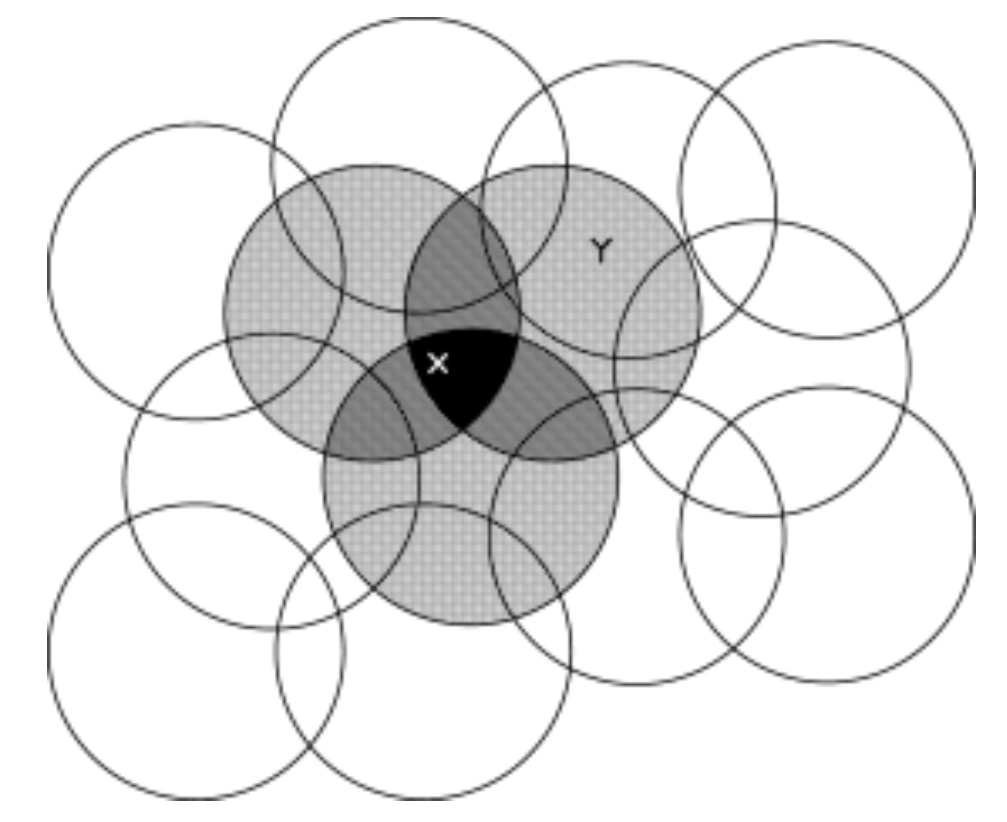
\includegraphics[width=0.5\linewidth]{images/coarsecoding1.png}
\caption[Generalization between points]{$X$ and $Y$ share 1 feature, as both points lie in the same receptive field, a circle. Thus, slight generalization from $X$ to $Y$ is possible. Source: \cite{Sutton1998ReinforcementIntroduction}.}
\label{fig:coarsecoding1}
\end{figure}
If the circles are small or large, generalization will be over respectively a short or large distance. The nature of the generalization is also affected by the shape of the features' receptive fields.  This can be seen in Figure~\ref{fig:coarsecoding2}. The fineness of discrimination is however only determined by the total number of features.
\begin{figure}[htb]
\captionsetup{width=0.8\textwidth}
\centering
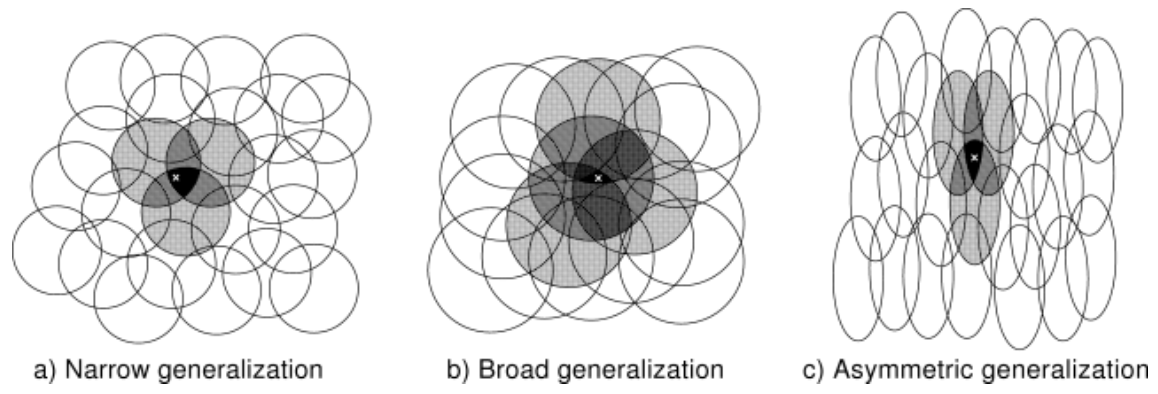
\includegraphics[width=0.8\linewidth]{images/coarsecoding2.png}
\caption[Shapes of receptive fields]{Generalization depends on the shape of the receptive fields of the features. When multiple features' receptive fields overlap, the generalization is broad and narrow when only few of them overlap. Source: \cite{Sutton1998ReinforcementIntroduction}.}
\label{fig:coarsecoding2}
\end{figure}

In tile encoding, a form of coarse encoding, the fields of the features are grouped into exhaustive partitions of the input space, called tilings. These tilings are defined by ranges of values for state attributes that they cover. For one specific tiling, the state can only lie in the ranges of 1 tile. As such, maximally one feature is active in each tiling and the total number of features present is always the same as the number of tilings. This allows us to set the step-size parameter $\alpha$ (used in formula \ref{eq:backview1}) in an easy, intuitive way. We can for example choose $\alpha = \frac{1}{m}$, where $m$ is the number of tilings. This results in exact one-trial learning. When the example $s_t \mapsto v_t$ is received, then the new value will be $V_{t+1}(s_t) = v_t$, whatever the prior value $V_t(s_t)$ was. For a slower change using for example $\alpha=\frac{1}{10m}$, one would move one-tenth of the way to the target in one update.\\
The weighted sum to make up the approximate value function is almost trivial to compute, as in tile coding only binary features are used. Instead of performing $n$ multiplications and additions, we compute the indices of the $m<<n$ present features and then add up the $m$ corresponding components of the parameter vector. The eligibility trace computation is also easier because the components of the gradient $\nabla_{\overrightarrow{\theta}} V_t(s_t)$ are either $0$ or $1$.\\
An easy to compute form of tilings are grid-like ones. Different tilings may also be used, ideally offset by different amounts. The width and shapes should match the width of generalization that is expected to be optimal. The denser the tiling, the more fine-grained the desired function can be, but also the greater the computational cost of updating. The width or shape of each tile must not be uniform or regular-shaped (like a square) however. One can also use stripes, diamond shapes, \dots To reduce memory requirements, hashing can be used. A large tiling can be collapsed in such way into a much smaller set of tiles. This hashing produces tiles consisting of non-contiguous, disjoint regions randomly spread throughout the state space, but that still form an exhaustive tiling.\\
Radial basis functions are a generalization of coarse coding that allows for continuous-valued features: in the interval $[0,1]$ instead of just $0$ or $1$. This way, we can reflect various degrees to which the feature is present. A typical RBF feature, $i$, has a Gaussian (bell-shaped) response $\phi_s(i)$ dependent only on the distance between the state and the feature's center state, $c_i$ and relative to the feature's width $\sigma_i$:
\begin{equation}
\phi_s(i) = e^{-\frac{||s-c_i||^2}{2 \sigma^2_i}}
\end{equation}
The advantage of this method is that they produce approximate functions that vary smoothly and are differentiable. The disadvantage is that $\sigma_i$ and $c_i$ must be tuned manually and that non-linear RBF networks are computationally complex.\\

\chapter{Deep learning}
\label{cha:deep_learning}
%Review by \cite{LeCun2015DeepLearning}.\\

As was briefly mentioned in Section~\ref{sub:rl:gfa}, artificial neural networks can be used as function approximators.
However, feedforward artificial neural networks may lack capabilities to represent complex functions and might be unusable for certain kinds of input. They also lack granularity and can be influenced by variance in the input that is irrelevant for the task (e.g.\ in a classification task, shifted objects in a picture should still be classified correctly). Because of this, they are not suitable for complex tasks like image recognition, unless an adequate feature extractor is applied first. Generic methods like kernel methods can be applied but are not guaranteed to work well for the task.\\
Generally, feature extractors need to be developed manually in order to represent the aspects of the input that are important. This, however, requires more work and requires knowledge about the domain and the task.\\

In contrast, deep learning methods are able to learn multiple levels of representations of raw data without human guidance.
Each level of features builds upon the previous one, starting from the input itself, and represents it in a more abstract way. These abstractions are generated as to recognize aspects of the input that are important for the task. Because of this, it is possible that small variations in the input have no influence on the abstraction and output.
As these abstractions are learned automatically, there is no need anymore to create internal representations manually, which require more work as it is different for every kind of task. The generated abstractions may also recognize useful patterns in the data that might not be intuitive to a human and would not have been represented using the hand-crafted features.\\

In deep learning, the important aspects of the input can be detected automatically by combining different modules that have different functions in order to get higher abstractions and to eventually generate output.
Most of these modules contain weights an can be trained, like explained in Section~\ref{sec:gradient_descent_and_backpropagation}.\\
Here, we explain artificial neural networks capable of learning representations using multi-dimensional arrays and sequential data, following the explanation by \cite{LeCun2015DeepLearning}.

\section{Convolutional neural networks}
Convolutional neural networks are neural networks that are inspired by the way the visual cortex of an animal works.
These networks get as input data in multi-dimensional arrays, such as 2-dimensional images with pixel intensities as the third dimension for example.\\
A convolutional neural network is structured as a series of stages, which are combinations of layers.
In the first stages, convolutional layers and pooling layers are used.
In a convolutional layer, units are organized in feature maps.
Each of these units is connected to a patch in the feature maps of the previous layer through a matrix of weights that is called the \emph{filter bank} or the \textit{kernel}.
The filter bank matrix then slides over the feature map, does an element-wise computation of the 2 matrices and sums the results.
The filter bank is then moved by a certain amount, called the stride.
All units in a specific feature map of a layer use the same filter bank.
An example of this process is shown in Figure~\ref{fig:cnnfilter}.
\begin{figure}[htb]
    \centering
    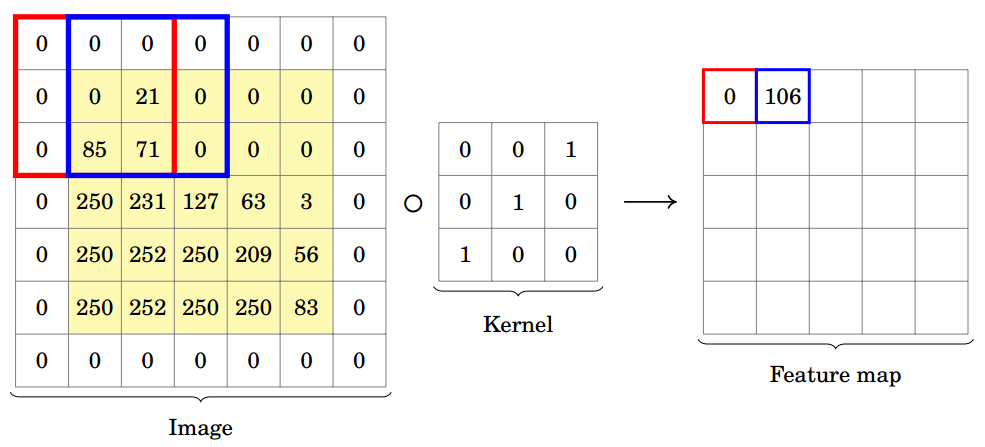
\includegraphics[width=.8\linewidth]{images/cnnfilter.png}
    \caption[An example of a 3-by-3 filter applied to an image]{An example of a 3-by-3 filter applied to an image. The filter is first applied using an element-wise computation and summation on the red square shown in the image, resulting in the value on the right. Then, because the stride is $1$, we move the filter one pixel to the right (shown in the blue square) and perform the same computation. Zeros are added in order to get a feature map of the same size as the input. Source: \cite{pavlovsky2017}.}
    \label{fig:cnnfilter}
\end{figure}

These filters are used because local groups of values may be correlated and as such may have the same weights. This reduces the amount of weights that need to be trained. Furthermore, certain concepts and local statistics (of images) may be invariant to the location. A certain pattern or motif in an image might appear in different places of the image but may have the same meaning.\\
The result of this convolutional operation (which is linear) operation is again a feature map and can then be passed to a non-linear function such as a \textit{ReLU}.\\

These convolutional layers are then combined with pooling layers. Instead of detecting local conjunctions of features from the previous layer, pooling tries to merge semantically similar features into one. This is necessary because the positions of features that form a motif are not exact and can vary somewhat. It may not matter for example that an object is close or far in an image.
To detect the motifs more reliably, we course-grain their features. The typical pooling units compute the maximum or average of a local patch of units in one or a few feature maps. The neighboring pooling units do the same for patches that are shifted by one or more rows and/or columns and as such creating an invariance to small shifts and distortions.\\
Popular convolutional networks, often using multiple layers of different types, include "AlexNet" \parencite{conf/nips/KrizhevskySH12}, "LeNet" \parencite{lecun-gradientbased-learning-applied-1998} and "GoogLeNet" \parencite{DBLP:journals/corr/SzegedyLJSRAEVR14}.\\
A typical layout of a convolutional neural network is shown in Figure~\ref{fig:cnnlayout}, while a hierarchy of features extracted using a convolutional neural network is shown in Figure~\ref{fig:cnnfeatures}.\\
\begin{figure}[htb]
    \centering
    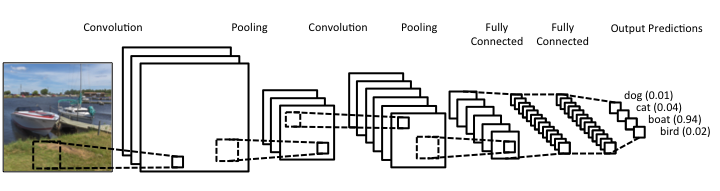
\includegraphics[width=\linewidth]{images/cnnlayout.png}
    \caption[Convolutional neural network layout]{Layout of a typical convolutional neural network, which uses convolutional layers, pooling layers and fully connected layers in order to detect an object in an image. Source: \url{https://www.clarifai.com/technology}}
    \label{fig:cnnlayout}
\end{figure}
\begin{figure}[htb]
    \centering
    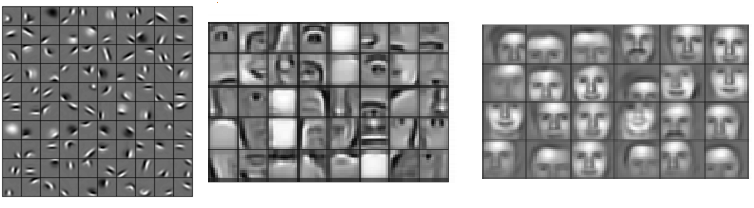
\includegraphics[width=\linewidth]{images/cnnfeatures.png}
    \caption[Convolutional neural network features hierarchy]{A hierarchy of features with as low-level features contours of faces. A more complex layer represents parts of faces. The final layer shows whole faces and can be used for classification or regression. Note that these features don't always have an intuitive meaning. Source: \cite{conf/icml/LeeGRN09}.}
    \label{fig:cnnfeatures}
\end{figure}

\section{Recurrent Neural Networks}
Recurrent neural networks (RNNs) are used to process sequential data such as speech and language. Here, an input sequence is processed one element at a time. The first RNNs used a state vector in their units that contains history about the past elements in the sequence. This is visualized in Figure \ref{fig:rnnunrolled}.
\begin{figure}[htb]
\centering
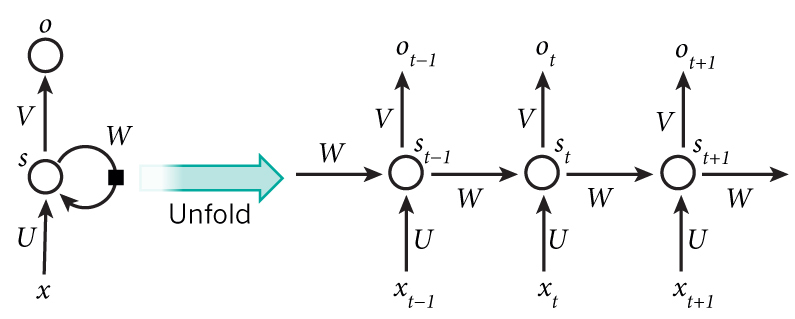
\includegraphics[width=0.8\linewidth]{images/RNN-unrolled.jpg} %source: http://www.wildml.com/2015/09/recurrent-neural-networks-tutorial-part-1-introduction-to-rnns/
\caption[Recurrent neural network]{A recurrent neural network in which each state (hidden unit) is passed to the next one. $x_t$ and $o_t$ are respectively the input and output at time step $t$. $s_t$ is the output of a hidden layer and depends on the input and the hidden unit at the previous time step: $s_t = U*x_t + W*s_{t-1}$. Note that the same weights $U$, $V$ and $W$ are used at each time step. Source: \cite{LeCun2015DeepLearning}.}
\label{fig:rnnunrolled}
\end{figure}
%The above diagram has outputs at each time step, but depending on the task this may not be necessary. For example, when predicting the sentiment of a sentence we may only care about the final output, not the sentiment after each word. Similarly, we may not need inputs at each time step. The main feature of an RNN is its hidden state, which captures some information about a sequence.

Training them was a problem because of the vanishing or exploding gradients, as these gradients either shrink or grow at every time step. Theoretical and empirical evidence has shown that it is hard for these kind of networks to store information long enough and that they have difficulties to learn the long-term dependencies \parencite{bengio1994learning}.\\ %Sources for this: http://people.idsia.ch/~juergen/SeppHochreiter1991ThesisAdvisorSchmidhuber.pdf and http://www-dsi.ing.unifi.it/~paolo/ps/tnn-94-gradient.pdf

To learn RNNs, we also need to change the backpropagation algorithm in order to handle with the different time steps. Here, the error (for one training example) is just the sum of the errors at every time step: $e = \sum_t e_t$. The adapted backpropagation algorithm, called backpropagation through time (BPTT), also just sums up the gradient at every time step for every set of weights:  $\frac{\partial E}{\partial W} = \sum_t \frac{\partial E_t}{\partial W}$. For the weights $U$ and $V$ of Figure \ref{fig:rnnunrolled}, the gradients are computed just as in normal backpropagation. For $W$ however, we depend on the previous state, which cannot simple be treated as a constant, and must be replaced as well. Because of this, we get:
\begin{equation}
\frac{\partial E_t}{\partial W} = \sum_{k=0}^t \frac{\partial E_t}{\partial \hat{y}_t} \frac{\partial \hat{y}_t}{\partial s_t} \frac{\partial s_t}{\partial s_k} \frac{\partial s_k}{\partial W}
\end{equation}
We see that training can be hard when the sequences are long, because we need to propagate back through the first time step.\\

For the \textit{tanh} and \textit{sigmoid} function, the derivative is $0$ at both ends. This means that the gradients in other layers will also go towards zero and for small values in the matrix multiplications the gradient values are shrinking exponentially fast and become nearly zero after a few time steps. Because of this, steps far away won't contribute much to what you're currently computing, and as such the long-term dependencies are small. If the values of the partial derivatives are high however, we could get exploding gradients. These are however easier to detect and solve, because the value of the gradients will be too high to be presented by a variable in the programming language. The problem can also easily be solved by restricting the value in a certain range.\\ %source: http://www.jmlr.org/proceedings/papers/v28/pascanu13.pdf
The problem of vanishing gradients can be solved by a better initialization of the weights, by regularization and by another non-linear function, namely the already explained \textit{ReLU}.
For this function, the derivative is either 0 (when $z<0$) or 1 ($\frac{\partial z}{\partial z} = 1$).\\

A way of solving this is using a long short-term memory. This is a combination of different units and has an explicit memory. One of the units has a connection with itself and is used to accumulate or forget the stored information. It can be learned using another unit to know when to forget something and when to remember past information.\\
First, the input is passed to an input gate $i_t$ that determines how much of the input to let through into the memory. By also both adding and forgetting a part, determined using a forget gate $f_t$, the internal memory is updated. An output gate $o_t$ then determines how much of the internal memory to output to the next layer.
The architecture of an LSTM cell is shown in Figure~\ref{fig:lstm}.
\begin{figure}[htb]
    \centering
    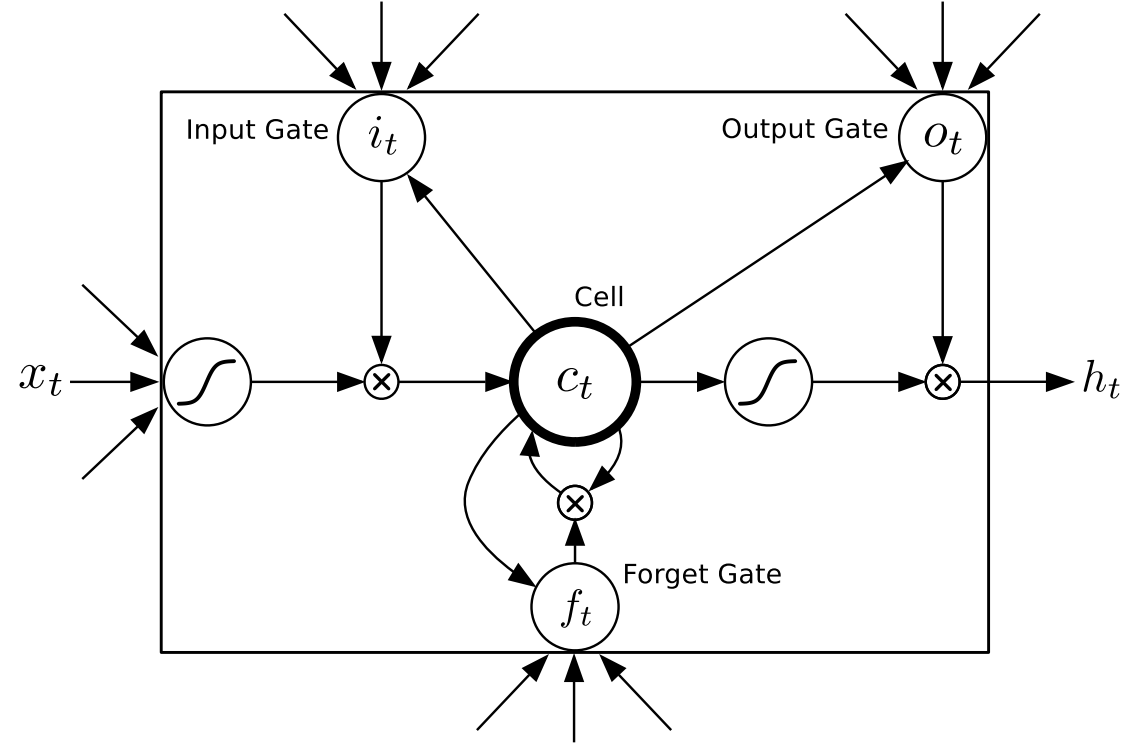
\includegraphics[width=.8\linewidth]{images/lstm.png}
    \caption[Long short-term memory cell]{The architecture of an LSTM cell. Source: \cite{journals/corr/Graves13}.}
    \label{fig:lstm}
\end{figure}
\\

Another kind of recurrent unit is the Gated Recurrent Unit (GRU), which was introduced by \cite{Cho2014LearningTranslation}. It is simpler than LSTM but yields similar results.
It also uses an internal memory, here called the \textit{hidden state} and denoted by $h$. An update gate $z$ determines how much of the previous memory we want to keep, depending on the previous hidden state and the input. A reset gate $r$ says how much of the previous hidden state we want to keep in the new hidden state, depending on the hidden state and the input. The new hidden state is then a combination of the partly "reset" previous hidden state and the input. The output is the sum of the previous hidden state and the new one, weighted by the reset gate.\\
By always setting the reset gate to $1$ and the update gate to $0$ we get again the classic RNN architecture.\\
The architecture of a GRU cell is visualized in Figure~\ref{fig:gru}.\\
\begin{figure}[htb]
    \centering
    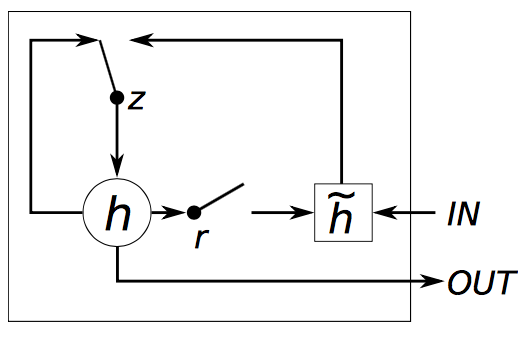
\includegraphics[width=0.6\linewidth]{images/gru.png}
    \caption[Gated Recurrent Unit cell]{Gated Recurrent Unit cell. Source: \cite{journals/corr/ChungGCB14}.}
    \label{fig:gru}
\end{figure}

Other networks with memory include a Neural Turing Machine, in which a tape-like memory is used from which the network can read or write.\\
Another kind is a memory network, in which a normal network is augmented by a associative memory.\\

\chapter{Deep reinforcement learning} % (fold)
\label{cha:deep_reinforcement_learning}
In deep reinforcement learning, deep learning methods are used to generalize over states and to approximate functions that are part of reinforcement learning algorithms.
Using this combination, we can learn to act in environments where the state is represented by a high-dimensional value, such as an image.
Again, multiple levels of representations are built. Here, these representations are built in order to perform better in an environment.\\
Besides dealing with high-dimensional inputs, deep reinforcement learning algorithms must also be able to overcome instability issues. These are caused by subsequent observations being correlated. When learning while acting in the environment, learned knowledge can also be overwritten when the data distribution changes (called "catastrophic forgetting"),  an issue that occurs for example when exploring a new part of the state space. Last, it is also possible that the function approximator parameters diverge.\\

First, we will discuss Deep Q-Network (DQN), which solves these problems by using a more stable target to learn on and learns on past experiences, leading to uncorrelated data. Afterwards, we will discuss Asynchronous Advantage Actor Critic (A3C). Instead of learning using past experiences, this algorithms obtains uncorrelated data and avoids catastrophic forgetting by learning in parallel with different actors on the same environment.

\section{DQN}
\label{sec:dqn}
A Deep Q-Network (DQN), presented in \cite{Mnih2015Human-levelLearning}, aims to combine deep learning with reinforcement learning.
It applies a convolutional neural network to high-dimensional sensory inputs such as the pixels of a game screen in order to approximate an action-value function $Q^{*}(s,a)$.
This is parametrized by the weights of the convolutional neural network, thus being $Q(s;a;\theta_i)$.
Past experiences are also reused and the Q value function used to select action is only periodically updated to the most recently learned one in order to reduce instability.\\

This instability is caused by using a nonlinear function to approximate the action-value function and by the correlation between subsequent observations.
Small changes in the $Q$ value can lead to big changes in the policy and because of that the data distribution and the correlations between the action-values $Q(s,a)$ and the target values $r+\gamma \max_{a'} Q(s',a')$ can also change a lot.
The action that is selected determines which states that will be observed next.

Experience replay solves the problem of having correlated subsequent observations and changing data distributions by randomizing used mini-batches of the data on which is learned.
In each iteration, these random mini-batches of saved experiences are used for applying Q-learning updates.
Experiences can be used multiple times, which results in an efficient use of the available data.\\
For the replay memory, all the encountered experiences can be used or only the $N$ most recent ones.
Here, however, it is possible that we forget experiences that may be important.
Because we use uniform sampling to determine which experiences to use, we also give no extra importance (i.e.\ more probability) to more useful experiences.

A second improvement is to only update the used target function every $C$ steps.
This helps to reduce the correlation between the action-value function values and the target values, as for example $Q(s_t, a_t)$ can have an influence on $Q(s_{t+1},a)$.
To do this, we copy the current network weights to obtain an action-value function $\hat{Q}$ to generate target values $y_j$.
By doing this, we add a delay between the time an update to $Q$ is made and the time the update affects the targets $y_j$, making divergence or oscillations much more unlikely.

The loss function used to update the weights of the parametrized action-value function is:
\begin{equation}
L_i(\theta_i) = E_{s,a,r,s' \sim U(D)} \left [ (r + \gamma \max_{a'} Q(s',a'; Q^{-}_i - Q(s,a;\theta_i)^2 \right ]
\end{equation}
Where $U(D)$ means that we take a uniformly random subset of the data set $D$. $\theta^{-}_i$ are the network parameters used to compute the target value. $\gamma$ determines the importance of future rewards. Instead of stochastic gradient descent, RMSProp is used here to update the weights.\\

The deep convolutional neural network gets as input the pixel colors of a game screen and has an output unit for every possible action. As such, we can compute the action-value function for every action when being in a certain state using only one forward pass.\\

To select an action, we can use the classic action selection policies such as $\epsilon$-greedy and softmax. Using these policies, we can learn off-policy because we do not always choose the action with the highest action-value. The value of respectively $\epsilon$ or $\tau$ in these mentioned policies can change over time to get closer to on-policy.\\

All rewards were clipped between -1 and 1 to limit the scale of derivatives and as such the amount of change of the weights. It also allows for using the same learning rate for multiple games.\\
% \todo{Better explain gradient descent step?}
The resulting pseudo-code can be seen in Algorithm~\ref{algo:dqn}.\\
\begin{algorithm}[htb]
\DontPrintSemicolon
Initialize replay memory D to capacity N\;
Initialize action-value function $Q$ with random weights $\theta$\;
Initialize target action-value function $\hat{Q}$ with weights $\theta^- = \theta$\;
\For{episode = 1, M} {
    Initialize sequence $s_1 = \{x_1\}$ and preprocessed sequence $\phi_1 = \phi(s_1)$\;
    \For{$t=1,T$} {
        With probability $\epsilon$ select a random action $a_t$\;
        otherwise select $a_t = \argmax_a Q(\phi(s_t),a;\theta)$\;
        Take action $a_t$ and observe reward $r_t$ and new image $x_{t+1}$\;
        $s_{t+1} \gets s_t,a_t,x_{t+1}$\;
        Preprocess $\phi_{t+1} \gets \phi(s_{t+1})$\;
        Store transition $(\phi_t,a_t,r_t,\phi_{t+1})$ in $D$\;
        Sample random minibatch of transitions $(\phi_j,a_j,r_j,\phi_{j+1})$ from $D$\;
        \eIf{episode terminates at step $j+1$} {
            $y_j \gets r_j$\;
        }{
            $y_j \gets r_j + \gamma \max_{a'} \hat{Q}(\phi_{j+1},a';\theta^-)$\;
        }
        Perform a gradient descent step on $(y_j - Q(\phi_j,a_j;\theta))^2$ with respect to the network parameters $\theta$\;
        Every $C$ steps reset $\hat{Q} \gets Q$\;
    }
}
\caption[Deep Q-learning with experience replay]{Deep Q-learning with experience replay. Source: \cite{mnih2013playing}.}
\label{algo:dqn}
\end{algorithm}

\section{Continuous control with deep reinforcement learning}
It is also possible to use an Actor-critic algorithm along with a replay buffer like in the DQN algorithm \parencite{Mnih2015Human-levelLearning}. This idea is presented by \cite{Lillicrap2015ContinuousLearning}
%Uses Actor-critic with replay and (slightly) different target value function.

For the critic, a function approximator with the following loss is used:
\begin{equation}
L(\theta^Q) = E_{s_t \sim \rho^{\beta}, a_t \sim \beta, r_t \sim E} \left [ (Q(s_t, a_t \vert \theta^Q) - y_t)^2 \right ]
\end{equation}
Where
\begin{equation}
y_t = r(s_t,a_t) + \gamma Q(s_t, \mu(s_{t+1}) \vert \theta^Q)
\end{equation}
$\mu(s_t \vert \theta^Q)$ is a function that specifies the policy by mapping states to actions.
It can be seen that using the loss function we have a critic that is learned using the Bellman equation, just like in Q-learning.\\

Instead of just copying the weights to the target value network every $C$ steps, we gradually move the target value network values towards the learned network values: $\theta' \leftarrow \tau \theta + (1-\tau) \theta'$ with $\tau \ll 1$.
This has the effect that target values can only change slowly.
However, although learning is slowed down, it can help to avoid divergence.\\

Most of the games have different scales for their state values.
Possible solutions are to change the hyperparameters for each game individually or to scale the states manually.
However, it is also possible to use a more general solution called batch normalization.
Here, we scale normalize each dimension across the samples in a minibatch in order to have unit mean and variance.
This minimizes the covariance shift during training.
To have more exploration, noise is added to the actor policy.
This noise is generated using the Ornstein-Uhlenbeck process.

\section{Asynchronous Methods for Deep Reinforcement Learning}
\label{sec:a3c}
In \cite{Mnih2016AsynchronousLearning} experience replay is not used because of memory and computation usage and because it is off-policy, which means that it learns from data generated by a policy that may already be outdated.
Instead, we use multiple agents (that use well-known reinforcement algorithms) that run in parallel but each running on a separate instance of the same type of environment.
These all run on a multi-core CPU (i.e.\ on only one computer).
Each of the agents use the same parameters $\theta$, but by using certain exploration policies, they are able to each explore a possibly different part of the state space.
It is possible to use a different exploration policy for each agent as to maximize the exploration of different states.
Each agent also calculates a gradient w.r.t.\ the parameters $\theta$ depending on its experience.
These gradients are accumulated and after a certain number of steps they are applied to the parameters $\theta$.
Because they are global, this update has an effect on all agents.
After an amount (possibly the same amount as for the gradient update) of steps, the target network parameters $\theta^{-}$ can also be updated using the current parameters $\theta$. A high-level overview of the architecture of the algorithm is shown in Figure~\ref{fig:a3carchitecture}.\\
\begin{figure}[htb]
    \centering
    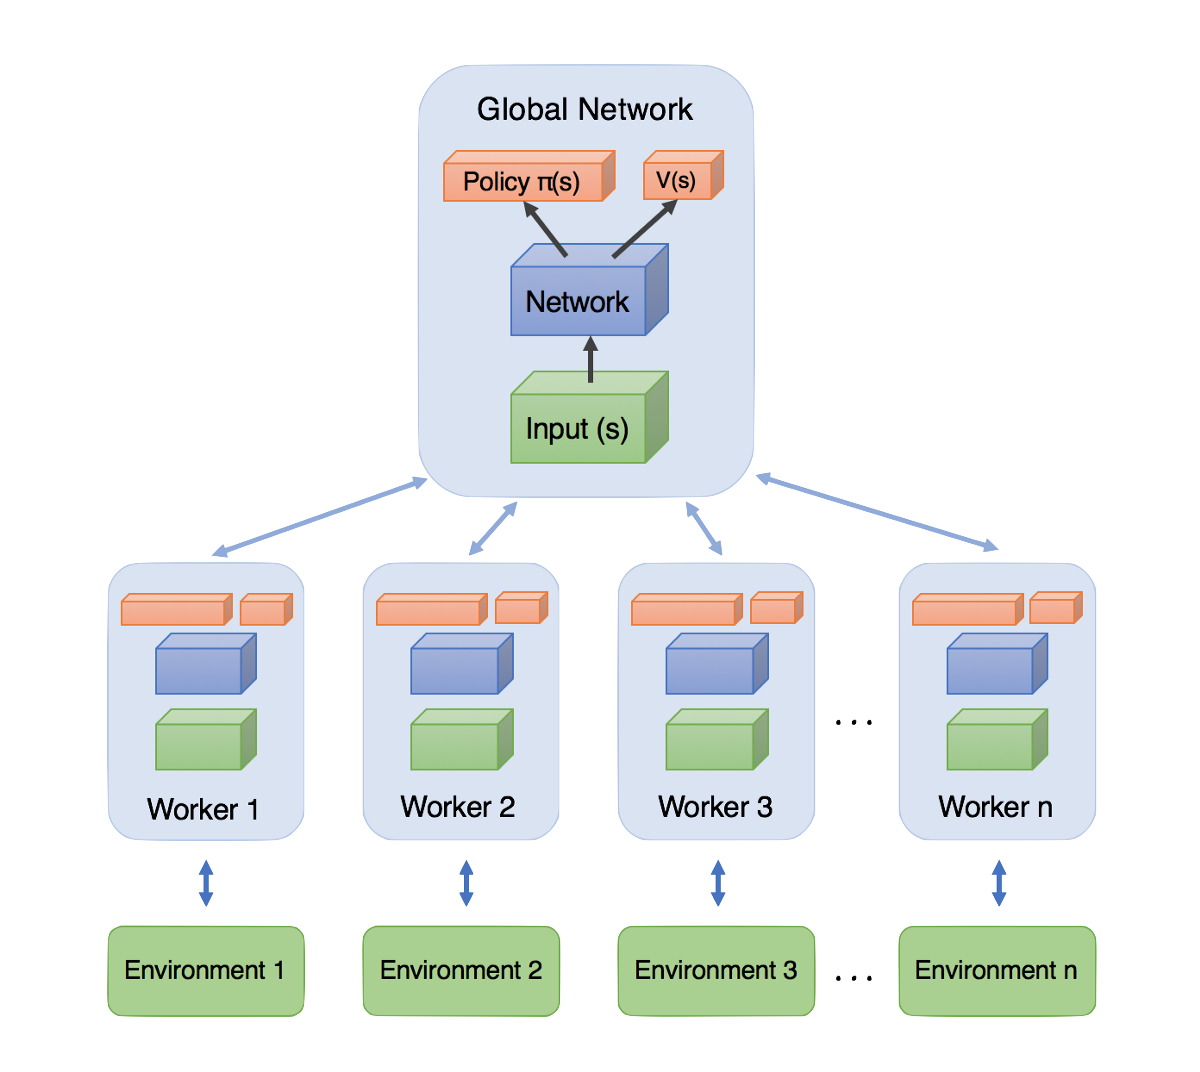
\includegraphics[width=.8\linewidth]{images/A3Carchitecture.png}
    \caption[High-level overview of the A3C algorithm]{High-level overview of the A3C algorithm. Each worker synchronizes its artificial neural network parameters with the global network and updates these based on input from the environment from which it is gathering transitions. Source: \cite{Juliani2016A3C}.}
    \label{fig:a3carchitecture}
\end{figure}
In $n$-step Q-learning and advantage actor-critic, a forward-view is used instead of the more commonly used backward view (which uses eligibility traces).
Forward view was found to be easier when training artificial neural networks with momentum-based methods and backpropagation through time.
To do this, we first compute a certain number of steps (or until the episode is over).
Then, the gradients are computed for each state-action pair encountered since the last update.
Each n-step update uses the longest possible n-step return resulting in a one-step update for the last state, a two-step update for the second last state, and so on for a total of up to the previously determined number of maximum allowed steps.
These accumulated gradients are then immediately applied to $\theta$.
This results in the pseudo-code shown in Algorithm~\ref{algo:a3c}.\\
\begin{algorithm}[htb]
\DontPrintSemicolon
\emph{// Assume global shared parameter vectors $\theta$ and $\theta_v$ and global shared counter $T=0$}\;
\emph{// Assume thread-specific parameter vectors $\theta'$ and $\theta'_v$}\;
Initialize thread step counter $t\gets 1$\;
\Repeat{$T > T_{max}$}{
    Reset gradients: $d\theta \gets 0$ and $d\theta_v \gets 0$\;
    Synchronize agent-specific parameters  $\theta'=\theta$ and $\theta'_v=\theta_v$\;
    $t_{start} \gets t$\;
    Initialize state $s_t$\;
    \Repeat{terminal $s_t$ \textbf{or} $t-t_{start}==t_{max}$}{
        Perform $a_t$ according to policy $\pi (a_t|s_t;\theta')$\;
        Receive reward $r_t$ and new state $s_{t+1}$\;
        $t \gets t + 1$\;
        $T \gets T + 1$\;
        }
        $R =
    \left\{
    \begin{array}{l l}
      0  \quad & \text{if $s_t$ is terminal}\\
        V(s_t,\theta'_v) \quad & \text{otherwise // Bootstrap from last state}
    \end{array}\right.$\;
    \For {$i \in \{t-1,\ldots,t_{start} \}$} {
        Accumulate gradients w.r.t. $\theta'$: $d\theta \gets d\theta + \nabla_{\theta'} \log\pi(a_i|s_i;\theta') (R - V(s_i;\theta'_v))$\;
        Accumulate gradients w.r.t. $\theta'_v$: $d\theta_v \gets d\theta_v + {\partial\left(R - V(s_i;\theta'_v)\right)^2}/{\partial \theta'_v}$\;
    }
    Perform asynchronous update of $\theta$ using $d\theta$ and of $\theta_v$ using $d\theta_v$\;
}
\caption[Asynchronous Advantage Actor Critic]{Asynchronous Advantage Actor Critic (A3C). Source: \cite{Mnih2016AsynchronousLearning}.}
\label{algo:a3c}
\end{algorithm}
% section deep_reinforcement_learning (end)

\chapter{Transfer learning}
%\cite{Taylor2009TransferSurvey}.
Transfer learning involves the use of experience gained when learning one or more tasks, to improve the performance on a different but related task. Each task is represented by a Markov Decision Process (MDP).\\  Here, we discuss a framework for transfer methods that can be used for reinforcement learning, closely following \cite{Taylor2009TransferSurvey}.\\

As already said, the transfer of knowledge always happens between one or more source tasks and a target task. First, an appropriate set of tasks must be selected. Afterwards, the transfer learning algorithm must learn how these source tasks are related to the target task. Then, the appropriate knowledge can be transferred.\\

\section{Transfer learning dimensions} % (fold)
\label{sub:transfer_learning_dimensions}
To be able to transfer knowledge, some assumptions must be made about the differences between the source tasks and the target task. This can be for example in the underlying dynamics of the environment, which can make the task harder or easier to solve, or different sets of possible actions at certain states.
These differences define between which type of source and target tasks knowledge can be transferred. The differences between the source task(s) and target task can also make the transfer of knowledge easier or harder, requiring the appropriate guidance by a human or a method that can overcome these differences in case of a fully autonomous transfer learner.\\
Multi-task learning is a special kind of task learning where the problems for the source and target tasks are drawn from the same distribution instead of having arbitrary source and target tasks. More specifically, the transition function is drawn from a fixed distribution of functions. For the mountain car environment, where an underpowered car must be driven up a hill, this may mean for example that the motor of the car differs in power in different tasks.\\

As was stated, first the set of source tasks needs to be selected. Again, this can be done by a human in case of a human-guided scenario. However, the selection may also be done by the agent itself. For example, it can learn multiple source tasks and then use them all for transfer.
Another possibility is to select the source tasks that are the most relevant and lead to highest performance for the target task.
The agent may also just aim to avoid negative transfer, such that the specific selection of source tasks does not worsen the learning performance for the target task.
The agent could also modify the source task(s) such that the transferred knowledge is the most useful in the target task.\\

Instead of just knowing that tasks are related, many methods also need to know how tasks are related, using task mappings. This is necessary to make the knowledge gained on the source tasks useful for the target task. Tasks may differ in state and action variables and the in the semantic meaning of them. In the mountain car environment, one can have a task where the goal is on the opposite side. As such, taking the action \texttt{Left} has a different meaning for these tasks. Actions in the two tasks must be mapped such that their effects are similar.\\
Again, these mappings can be provided by a human or they can be learned by the agent. Note that these mappings may be partial and not every action in the source task is mapped to an action in the target task or vice-versa. For the state space, it is also possible to map the states themselves instead of the state variables.\\
In multi-task learning, states and variables are the same and have the same meaning. Because of this, no task mappings are necessary in multi-task learning.\\

Task learning methods can also differ in the type of knowledge that is transferred between source and target tasks. This knowledge can be for example an action-value function, transitions or policy gradient parameters. For tasks that are closely related, detailed knowledge may be useful. Otherwise, high-level information may result in a better learning performance. The type of knowledge that is transferred can also depend on the type of source and target tasks and on the task mappings.\\

Last, the task learning method may also restrict which reinforcement learning algorithms that can be used. It is possible for example that only a class of reinforcement learning algorithms or only one specific reinforcement learning algorithm can be used with the task learning method or that the algorithm is the same for both the source and target tasks. Ideally, the reinforcement learning algorithms can be chosen freely and may be selected based on the characteristics of the tasks at hand.\\
% section transfer_learning_dimensions (end)

\section{Metrics}
\label{sub:tl_metrics}
Several metrics exist to evaluate the learning performance and solution quality of transfer learning algorithms. Generally, one metric does not give a complete representation of the overall performance of the algorithm. Because of this, often multiple metrics are used.\\
Here we will list the most popular ones:
\begin{itemize}
    \item \textit{Jumpstart}: This is the initial improvement that the target task has over an algorithm that does not use knowledge transfer. However, little to no learning has occurred yet. Because of this, learning performance can't be measured. The metric also does not give an indication about the final performance, i.e.\ the performance after having learned.
    \item \textit{Asymptotic performance}: This is the opposite of \textit{jumpstart} performance and measures the performance improvement after having learned the target task or during the last time steps of the algorithm. However, this is hard to measure because one has to know when the task learning algorithm converged. Furthermore, the task learning algorithm and the algorithm that does not use knowledge transfer may require a different training time in order to converge.
    \item \textit{Total reward}: This is the total reward that the algorithm has accumulated during learning, i.e.\ the area under the learning curve. In case of improvement, this area is bigger than when transfer learning isn't used. This can be achieved when the transfer learning algorithm has a higher learning rate.
    However, convergence is again an issue here. An algorithm that learns slower and thus takes more time to converge may accumulate a higher total reward than a faster algorithm, although the latter may even reach a higher performance. This metric is only useful for tasks that always have the same duration.
    \item \textit{Transfer ratio}: This is the ratio of the total reward improvement that the transfer learning algorithm has over the other algorithm. Because it uses the \textit{total reward} metric, it suffers from the same issues. Furthermore, it is also influenced by the reward structure. For example, an agent always receiving a reward of $+1$ at the end of the episode may result in a different ratio.
    \item \textit{Time to threshold}: This measures the time needed to reach a pre-defined performance. A transfer learning algorithm may need less time to reach this threshold. The threshold needs to be defined manually and depends on the task domain and learning method.
\end{itemize}
A graph with 4 of the 5 metrics is shown in Figure~\ref{fig:TLmetrics}.
\begin{figure}[htb]
    \centering
    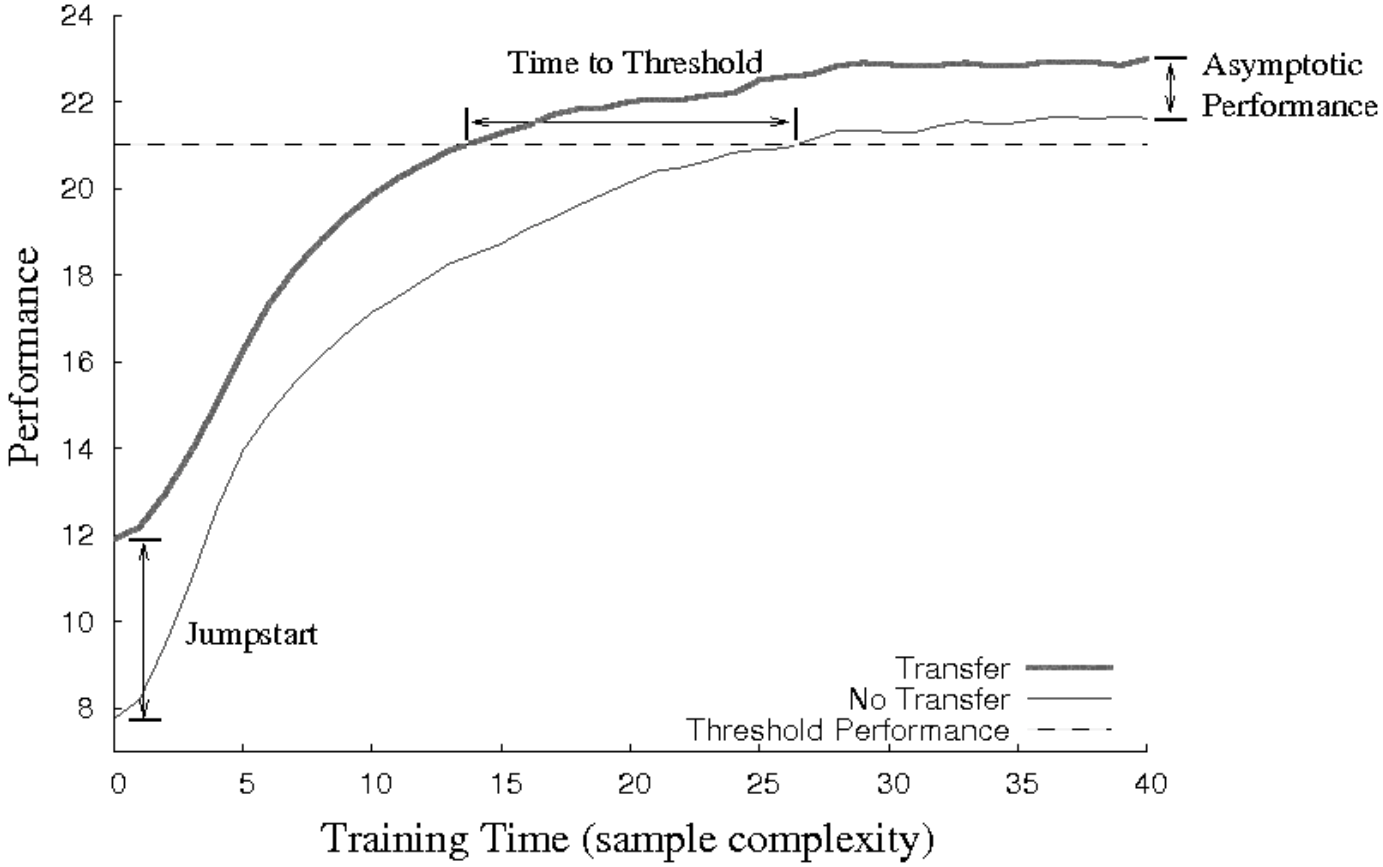
\includegraphics[width=.9\linewidth]{images/tlmetrics.png}
    \caption[Transfer learning metrics]{A graph comparing the \textit{jumpstart}, \textit{time to threshold} and \textit{asymptotic performance} metrics between the algorithm that uses knowledge transfer and the one that does not use it. Note that here the transfer learning algorithm performs better on all three metrics. It can also be seen that the total reward is higher. Source: \cite{Taylor2009TransferSurvey}.}
    \label{fig:TLmetrics}
\end{figure}
Instead of comparing the transfer learning algorithm with an algorithm that does not use knowledge transfer, it is also possible to compare the algorithm with the performance of humans (by averaging their performances).
However, metrics must be chosen carefully such that they do not favor the algorithm or the human and that they cannot be abused.

\section{Related work}
% Types of knowledge that is transferred: Value functions, features extracted from value functions, heuristics, policies
% Different representation types: Graphs, relational representation, tables

% Representation transfer
    % options

% separation in subtasks

% Relational RL

% transferring instances
% transferring advice/preferences
Transfer learning methods for reinforcement learning can be divided into 2 groups: methods that use task mappings and methods that do not.
We will mostly discuss methods that do not use task mappings as our approach also does not use task mappings.\\

In one of the earliest works of transfer learning used for reinforcement learning \parencite{conf/ijcai/SelfridgeSB85}, the transition function was gradually changed as to make the task harder.
A \emph{cart-pole} task was used where the pole was long and light at first, but was made shorter and heavier over time.
The total time spent learning on the sequence of gradually modified tasks was shorter than when trying to solve the hardest task directly.\\

Later work was generally focused on transferring from one source task to a target task, while in recent research, most of the times a more general scenario with possibly multiple source tasks is considered.
The approaches that we will further discuss mostly focus on transferring from multiple source tasks instead of just one.
We do this because our approach also allows the use of multiple source tasks.
Furthermore, the  discussed algorithms that can use multiple source tasks generally also allow just one source task from which to transfer knowledge.\\

One approach, presented in \cite{lazaric2008transfer}, is to transfer transitions (also called \textit{instances} or \textit{samples}) gathered from the source tasks to the target task.
However, transitions may not be useful if the target tasks differs too much from the source tasks.
To solve this, transitions from source tasks are chosen based on the similarity of these tasks to the target task.
After having trained on the source tasks and collected transitions, we also collect a few transitions from the target task.
The similarity between a source task and the target task is then the probability that the transitions of the target task were generated by an approximated model of the source task.

\cite{Ammar2014} also focus on the problem of selecting the appropriate source tasks from which to transfer knowledge.
Here, however, a Restricted Boltzmann Machine \parencite{Smolensky1986} is used in order to generate a model of a source tasks that yields features that are relevant for characterizing the task.
The model, generated using transitions of the source task, then tries to reconstruct samples of the target task.
The similarity of a source and target task can then be assessed using the difference of the reconstructed transitions and the real transitions of the target task.
Note however that the state and action spaces of the source tasks and target task needs to be the same.\\

Another possibility is to transfer a representation, for example by transferring features extracted from the states. In this case, characteristics are inferred from multiple source tasks.
In \cite{Bernstein99reusingold}, policies are averaged and can be applied for $n$ time steps on all states.
This combination of a policy, time steps to execute and states is called an option.
The reasoning is that actions that are used a lot in a state in source tasks may also be useful in the target task. In \cite{perkins1999using}, these options are provided on beforehand.
The agent then learns a single action-value function over these options using all the source tasks.
These options along with the action-value function can then be transferred and used for the target task.\\

Instead of using a single policy or action-value function, one can also collect a library of policies and select one to use probabilistically, depending on the expected reward. This approach is presented in \cite{fernandez2006probabilistic,fernandez2013learning}. At every time step, the algorithm can choose to use one of the source task policies, use the current best target task policy or to randomly explore. As the probabilities depend on the gained rewards, after some time more useful policies are exploited more often. This method only works however for tasks where only the goal state in a maze is different.\\

In \cite{conf/cira/TanakaY03} action-value functions are transferred instead of policies and statistics about those functions are exploited.
More specifically, the average and standard deviation of the value each state-action pair is calculated.
In the target task, the action-value function for each state-action pair is then instantiated to the average for that pair for the source tasks.
The standard deviation is used in order to prioritize updates for state-action pairs that are far from the average.
Besides this, states-action pairs that fluctuate often within an episode are also prioritized.\\

\cite{journals/ml/FosterD02} try to extract sub-tasks across multiple source tasks.
Optimal policies are then learned for each of these sub-tasks and pieced together.
In this case, the environment was a maze and tasks differ in their goal in the maze.
Value functions can then be learned on parts of the maze.
Less learning for the target task is then required because most of the already learned sub-tasks can also be used for the target task.\\

Most methods focus on problems with a discrete state and action space. However, other methods exist that can be applied on problems with a continuous state and action space.
Here, function approximation is always required. \cite{walsh2006transferring} group states encountered in the source tasks and treat them as being one and the same state.
This abstraction along with the value function learned on this abstraction can then be transferred and used for learning the target task.\\
\cite{lazaric2008knowledge} also groups states of the source tasks, but does this by adjusting parameters of a function approximator to build features.
Only a small set of features are searched while still being able to learn useful value functions. The learning process for the tasks is executed in parallel.
Again, after learning the source tasks, the parameters of the function approximator and the value functions are transferred.

2 other approaches use a hierarchical Bayesian model. They use this to find parameters that make up the dynamics and reward function of a problem. In \cite{sunmola2006model}, transitions of source tasks are used as a prior to find parameters for models.
After getting transitions from the target task, the most probable model for the target task transitions is transferred and used.\\
\cite{conf/icml/WilsonFRT07} use a similar approach, but they do not make a distinction between source and target tasks. Instead, problems (MDPs) are executed sequentially and models are built using an already acquired set of transitions and models of previous tasks.\\

In \cite{Isele2016UsingLearning}, a multi-task learning method is presented that learns tasks simultaneously by using a predefined description for each task.
When a new task arrives along with its features, obtained from its task descriptor, a policy can be generated that immediately results in a good performance, even though the algorithm was not applied on that task before and the task descriptor, task order and task distribution were not known on beforehand. This is called \textit{zero-shot learning}.
As such, knowledge transfer can take place without the need of training data to identify relationships across tasks.
For each subsequent task, the policy and feature vector are iteratively improved.\\
%factorization: ontbinding in factoren: bijv. 15=3*5
First, it is assumed that the policy parameters for every task $t$ can be factorized using a shared knowledge base $L \in \mathbb{R}^{d \times k}$: $\theta^{(t)} = Ls^{(t)}$. $s^{(t)} \in \mathbb{R}^{(k)}$ are the sparse coefficients over the basis, i.e.\ the latent representation of the policy's parameters for task $t$. $L$ is able to capture relationships among policies as this is used to compute every policy, whereas there is a sparse representation for computed for each task separately.\\
The features of the task are obtained by (possibly non-linear) feature extractors applied on the descriptor of the task: $\phi(m^{(t)}) \in \mathbb{R}^{d_m}$.
These features can also be linearly factorized using another shared knowledge base $D \in \mathbb{R}^{d_m \times k}$: $\phi(m^{(t)}) = Ds^{(t)}$, where the same sparse representation is used as the one used to compute the policy.
Both knowledge bases provide information about the task and because of this they share the same coefficient vectors $S$.
We then use coupled dictionary optimization techniques from the sparse coding literature to optimize these dictionaries.
The dictionaries updated iteratively based on trajectories sampled from the current task.\\
When a new task arrives along with its task descriptor, we search for the coefficients $s^{(t_{new})}$ that minimize the difference between the extracted features and the reconstruction of it using the shared knowledge base $D$.
Using these coefficients, we can compute the policy parameters using $\theta^{(t_{new})} = Ls^{(t_{new})}$. Afterwards, we can iterate again to improve the sparse representation and the knowledge bases.\\

Together with the interest in deep reinforcement learning \parencite{Mnih2015Human-levelLearning,Mnih2016AsynchronousLearning}, the interest in its application to transfer learning also grows.
In \cite{DBLP:journals/corr/ParisottoBS15}, the algorithm, Actor-Mimic Network (AMN), learns the $Q$ function for source tasks from an expert for each specific task (in this paper a DQN that was trained until convergence).
Note that only one set of parameters (and thus one artificial neural network) is used to learn on all the source tasks.
As can be seen, this is supervised learning (more specifically regression) with the output of the expert's network as target value.
As input, both the expert and the AMN can be used to sample trajectories.
Besides mimicking using the expert's output, the AMN also tries to mimic the hidden layer activations of the expert's network.
This is done by adding a loss in function of the difference between the hidden layer activations of the expert network and the activations of the AMN.
Intuitively, this gives insight to the AMN, also called to student, why it should act in a specific way, in addition to telling how it should act.
After learning for a pre-determined number of frames on each task, the weights of the AMN are transferred to a DQN and the algorithm trains on an unseen target task.
Note that each task is a different kind of task here (i.e.\ the state space, action space, transition function and reward function can be different).
However, the algorithm can also be applied to tasks with the same state and action space.

% Progressive neural networks
In contrast to the previous algorithm, Progressive Neural Networks \parencite{Rusu2016} use A3C to learn tasks.
However, the focus here is on avoiding catastrophic forgetting, which causes previously learned weights to be overwritten when there is a different distribution in the data.
In this case, this means that we are learning a different task.
To solve this problem, a different set of artificial neural network weights is used for each task.
Knowledge is transferred using lateral connections from neurons of artificial neural networks used for previously learned tasks.\\
After a task is learned, the weights of the used artificial neural networks are kept fixed.
When a new task has to be learned, a new artificial neural network is instantiated, with each neuron being both the result of its own knowledge and that of previous tasks:
\begin{equation}
    h^{(k)}_i = f \left ( W^{(k)}_i h^{(k)}_{i-1} + \sum_{j<k} U^{(k:j)}_i h^{(j)}_{i-1} \right )
\end{equation}
Where $h^{(k)}_i$ is the output for layer $i$ of task $k$, $f$ is an element-wise activation function, $W^{(k)}_i$ is the weight vector for layer $i$ of task $k$ and $U^{(k:j)}_i$ are the lateral connections from layer $i-1$ of task $j$ to layer $i$ of task $k$.\\
The algorithm learns both its own weights and its lateral connections from the previous tasks.
Thus, it can decide which knowledge from previous tasks is useful.
However, it is not necessary to use this knowledge from previous tasks, as they may not be similar enough for the current task.
The task also cannot be influenced by future tasks, as it has no lateral connections from them.\\
A limitation of this algorithm is that a large amount of memory is required because each task has its own set of weights. It is also reported that only a fraction of those weights is utilized.

\chapter{Proposed algorithm}
\label{cha:proposed_algorithm} % (fold)
Our approach only uses a latent basis over the policy space instead of using one over the policy space and another one over the descriptor space like in \cite{Isele2016UsingLearning}.\\
Again, for a task $(t)$, we can reconstruct the policy using the shared basis $L$ and the sparse coefficients over this basis for that specific task $s^{(t)}$: $\theta^{(t)} = Ls^{(t)}$, with $\theta^{(t)} \in \mathbb{R}^d$, $L \in \mathbb{R}^{d \times k}$ and $s^{(t)} \in \mathbb{R}^k$.\\
The architecture of the network used for one task is visualized in Figure~\ref{fig:algonn}.
\begin{figure}[htb]
    \centering
    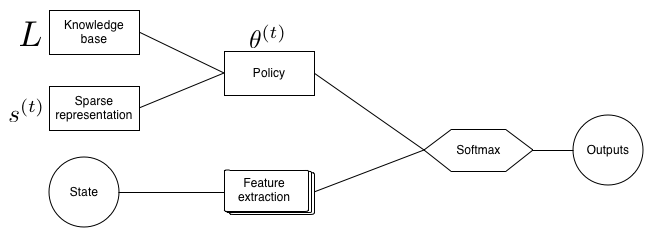
\includegraphics[width=\linewidth]{images/knowledge_transfer.png}
    \caption[Artificial neural network architecture used in our approach]{Artificial neural network architecture used in our approach. The sparse representation $\theta^{(t)}$ is different for every task $(t)$, while the same knowledge base is used for every task.}
    \label{fig:algonn}
\end{figure}

The source tasks can be learned in two ways. They can be learned either sequentially or in parallel.
In the sequential way, we collect trajectories and calculate the gradients for every task after another. These gradients include both those for the sparse representation and for the knowledge base. They are calculated for every episode of a task like in the \texttt{REINFORCE} algorithm (explained in Section~\ref{sub:rl_policy_gradient}), i.e. with likelihood ratios using discounted rewards as a sample for the $Q$ values of the policy.\\
After evaluating every task, we sum and apply all of their gradients. The learning process for the source tasks then stops when a certain number of updates have been applied.\\
In the parallel way, all source tasks are learned at the same time, each executing a certain number of updates. Trajectories are collected for each task continuously and its gradients are applied immediately after they are calculated. This means that they are not first summed up like in the sequential method.\\
The resulting pseudo code for the source tasks learned using the parallel method can be seen in Algorithm~\ref{algo:ownsource}.\\
\begin{algorithm}[htb]
\DontPrintSemicolon
\emph{// Assume global knowledge base $L$ and global shared counter $T \gets 0$}\;
% \emph{// Assume thread-specific parameter vector $\theta_g'$}\;
Initialize thread-specific parameter vector $\theta^{(t)}$\;
Initialize thread step counter $t\gets 1$\;
\Repeat{$T > T_{max}$}{
    $\theta^{(t)} \gets Ls^{(t)}$\;
    Reset gradients: $d\theta^{(t)} \gets 0$\;
    % Synchronize agent-specific parameters  $\theta_g' \gets \theta_g$\;
    $t_{start} \gets t$\;
    Initialize state $s_t$\;
    \Repeat{terminal $s_t$ \textbf{or} $t-t_{start} = t_{max}$}{
        Perform $a_t$ according to policy $\pi(a_t \vert s_t;\theta^{(t)})$\;
        Receive reward $r_t$ and new state $s_{t+1}$\;
        $t \gets t + 1$\;
        $T \gets T + 1$\;
        }
    \For {$i \in \{t-1,\dots,t_{start} \}$} {
        %Accumulate gradients w.r.t. $\theta'$: $d\theta \gets d\theta + \nabla_{\theta'} \log\pi(a_i|s_i;\theta') (R - V(s_i;\theta'_v))$\;
        Accumulate gradients w.r.t. $\theta^{(t)}$: $\theta^{(t)} \gets \theta ^{(t)}+ \alpha \nabla_{\theta^{(t)}} \log \pi_{\theta^{(t)}}(s_t,a_t)v_t$\;
    }
    Perform asynchronous update of $\theta^{(t)}$ using $d\theta^{(t)}$\;
}
\caption[Asynchronous knowledge transfer agent for a source task]{Asynchronous knowledge transfer agent for a source task.}
\label{algo:ownsource}
\end{algorithm}

After learning the source tasks, the knowledge base that they jointly learned is transferred to the target task. This task then separately learns and executes updates for a number of episodes. The pseudo-code for the target task is shown in Algorithm~\ref{algo:owntarget}.\\
\begin{algorithm}[htb]
\DontPrintSemicolon
\emph{// Assume global knowledge base $L$}\;
Initialize task-specific sparse representation $s^{(t)}$\;
Initialize thread step counter $t\gets 1$\;
\Repeat{$T > T_{max}$}{
    $t_{start} \gets t$\;
    Initialize state $s_t$\;
    \Repeat{terminal $s_t$ \textbf{or} $t-t_{start} = t_{max}$}{
        Perform $a_t$ according to policy $\pi(a_t|s_t;L  s^{(t)})$\;
        Receive reward $r_t$ and new state $s_{t+1}$\;
        $t \gets t + 1$\;
        }
    \For {$i \in \{t-1,\dots,t_{start} \}$} {
        %Accumulate gradients w.r.t. $\theta'$: $d\theta \gets d\theta + \nabla_{\theta'} \log\pi(a_i|s_i;\theta') (R - V(s_i;\theta'_v))$\;
        Accumulate gradients w.r.t. $s^{(t)}$: $s^{(t)} \gets s^{(t)} + \alpha \nabla_{s^{(t)}} \log \pi_{s^{(t)}}(s_t,a_t)v_t$\;
    }
    Perform update of $s^{(t)}$ using $ds^{(t)}$\;
}
\caption[Knowledge transfer agent for the target task]{Knowledge transfer agent for the target task.}
\label{algo:owntarget}
\end{algorithm}
% section proposed_algorithm (end)

\section{Experimental setup}
Experiments were executed on variations of the \textit{Cart-pole} environment and on variations of the \textit{Acrobot} environment.\\

In the 2-dimensional Cart-Pole environment, a pole is placed vertically on a cart. The goal in this environment is to keep the pole balanced vertically (i.e. keep the angle of the pole between thresholds) and to keep the cart between 2 borders.
The state is defined by 4 continuous-valued attributes: the position of the cart, the velocity of the cart, the angle of the pole and the angular velocity of the pole.
A discrete value of $1$ is given as a reward each time the pole is balanced and the cart is between bounds.
The episode ends either when these requirements are not fulfilled anymore or 200 steps have been executed.
An agent can either move left or right. It can't stay at its current position.
The environment is visualized in Figure~\ref{fig:cartpole}.
\begin{figure}[htb]
    \centering
    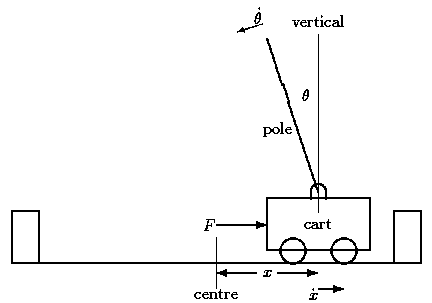
\includegraphics[width=.6\linewidth]{images/cartpole.png}
    \caption[Cart-Pole environment]{Cart-Pole environment. $F$ is the force applied to the cart when taking an action. $x$ is the distance of the cart from the center and $\dot{x}$ is its velocity. $\theta$ is the angle of the pole and $\dot{\theta}$ refers to its angular velocity. Source: \cite{grant1990modelling}.}
    \label{fig:cartpole}
\end{figure}
For executing the experiments, an implementation of this environment by \cite{Brockman2016OpenAIGym} was used.\\

The goal in the \textit{Acrobot} environment, visualized in Figure~\ref{fig:acrobot} is to swing up  the tip of 2 joined arms above a certain point \cite{spong1995swing}.
This can be done by applying a force on the joint between the 2 arms.
However, this force is not enough to fulfill the goal immediately. Instead, the actuator must apply force to the left and to the right to build up enough speed to get above the horizontal threshold.
The state consists of the angle and angular velocity of both arms. One can either move the joint clockwise, counter-clockwise or do nothing.
An episode stops either when the tip of the outermost arm is above the threshold or when 500 steps have been executed in the episode.
The goal is to minimize the amount of steps necessary to reach the threshold.
\begin{figure}[htb]
    \centering
    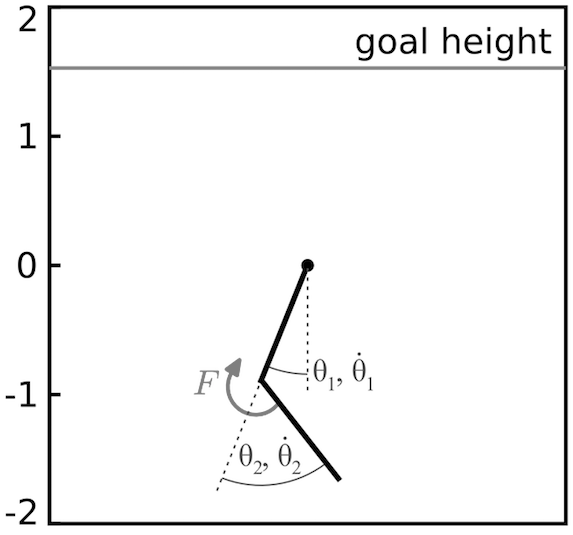
\includegraphics[width=.7\linewidth]{images/acrobot.png}
    \caption[Acrobot environment]{Acrobot environment. $\theta_1$ and $\dot{\theta_1}$ are respectively the angle and angular velocity of the arm attached to the central fixed point. $\theta_2$ and $\dot{\theta_2}$ are respectively the angle and angular velocity of the outermost arm. Source: \cite{fremaux2013reinforcement}}
    \label{fig:acrobot}
\end{figure}

In the experiment, first a number of environments are randomly generated. We try to learn with both 5 and 10 environments.
The environment for each task can differ for a predefined number of attributes, of which the values can each be in a certain range. For a cart-pole task, these are the mass of the cart, the mass of the pole and the length of the pole.\\
Then a number of source tasks were learned that can update both the shared knowledge base and their own sparse representation. After a number of epochs, i.e. updates to these variables, we stop with learning these tasks.
Instead, we learn to solve a new task, the target task, for which we hadn't learned its sparse representation yet. Here however, only the sparse representation can be updated and not the shared knowledge base.\\
This learning process is repeated 100 times, each time using a different set of environments and thus problems to solve.\\
Afterwards the rewards are averaged over all the runs.\\
Trajectories for both sets of tasks contained of maximally 200 or 500 steps depending on the type of environment. This could be less in case the environment was in an end state. In case of the cart-pole environment, this can mean for example that the cart tried to cross the left or right border or that the pole fell down.\\
Hyperparameters, such as the learning rate of neural networks, were chosen by iteratively executing the previously mentioned experiment. Possible values for each hyperparameter were chosen manually.

\chapter{Conclusions}

We presented an algorithm suitable for learning in parallel or sequentially on a set of source tasks.
These task share a knowledge base, but they also have their proper sparse representation.
The learned knowledge can then be transferred to the target task with the goal of having an increased performance over an algorithm that does not use prior knowledge.\\

In our experiments, we found that source tasks learned in parallel learned faster than when they were learned sequentially.
In the parallel version, changes to the shared knowledge base are applied immediately instead of summing them and applying the changes after all source tasks have been evaluated.\\

We also discussed to use of feature extraction applied to the input, which is in this case the state of an environment.
For the cart-pole environment, no feature extraction was necessary and even slowed down learning.
However, environments with a high-dimensional input space generally require feature extraction in order to obtain the relevant aspects of the input.\\

Our algorithm has better performance on the target task than when just using the \textit{REINFORCE} algorithm on it.
Our algorithm learns faster and is able to receive higher rewards.
The performance is even better when we transfer the sparse representation from a randomly chosen source task to the target task.
The algorithm then only needs to tune the sparse representation for it to work on its own task.\\

To see if multiple source tasks are really necessary, we compared our algorithm with the \textit{REINFORCE} algorithm where it learns on a single source task and transfers all its knowledge to the target task.
Although the asymptotic performance was similar, our algorithm learned better on the source tasks and has a higher jumpstart performance.\\

We can conclude that it is beneficial to learn on multiple source tasks in parallel and transfer knowledge learned on these tasks to the target task.

\section{Future work} % (fold)
\label{sec:future_work}
Most of the experiments in this thesis did not use feature extraction, as it was not necessary for the environments that were used. It would be interesting to execute experiments with an environment where feature extraction is necessary. This would require more complex artificial neural networks such as convolutional neural networks.\\

Furthermore, one could explore the use of this algorithm to transfer knowledge between different types of environments. For example, one could share knowledge between \textit{cart-pole} and \textit{acrobot} environments. This would require the artificial neural network to process inputs of different shapes and to output actions of different action spaces. For this, task mapping may be necessary to cope with those differences.
% section future_work (end)

\backmatter
\begin{appendices}
\chapter{Experiment details}
\section{Data collection} % (fold)
\label{sec:data_collection}
For each agent, transitions on which to learn were collected in the same way. In each iteration, $5000$ transitions have to be collected. To do this, we keep executing actions and saving the transitions until this threshold is reached. When an end state is reached before reaching this threshold, we reset the environment and keep executing actions.
% section data_collection (end)
\section{Artificial neural network parameters} % (fold)
\label{sec:artificial_neural_network_parameters}

% section artificial_neural_network_parameters (end)
% \begin{itemize}
%     \item number of layers and units
% \end{itemize}
Weights are initialized using values drawn from a truncated normal distribution with mean $0$ and standard deviation $0.02$.
This means that we draw values from a normal distribution with the same mean and standard deviation, except that only values maximally 2 standard deviations away from the mean can be drawn.\\
To update weights, I used \textit{RMSProp}, described in Section~\ref{ssub:different_weight_updates}.
The following hyperparameters were always used for both the sequential and the parallel version of the algorithm and for \textit{REINFORCE}:
\begin{itemize}
    \item $\epsilon = 10^{-9}$
    \item $\alpha = 0.05$
    \item $\gamma = 0.9$
\end{itemize}

\section{Environment parameters} % (fold)
\label{sec:environment_parameters}
Here we describe the range of possible values for each parameter of the \textit{cart-pole} and \textit{acrobot} environments.
To generate an environment, each parameters is drawn from a uniform distribution with possible values in the defined range.
For the \textit{cart-pole} environment, we have:
\begin{table}[H]
    \centering
    \begin{tabular}{l|cc}
    \hline
    \textbf{Parameter name} & \textbf{minimum} & \textbf{maximum} \\
    \hline
        Pole length & $0.01$ & $5.0$ \\
        Pole mass & $0.01$ & $5.0$ \\
        Cart mass & $0.01$ & $5.0$ \\
    \hline
    \end{tabular}
\end{table}
For the \textit{acrobot} environment, we have:
\begin{table}[H]
    \centering
    \begin{tabular}{l|cc}
    \hline
    \textbf{Parameter name} & \textbf{minimum} & \textbf{maximum} \\
    \hline
        Length of link 1 & $0.2$ & $2.0$ \\
        Length of link 2 & $0.2$ & $2.0$ \\
        Mass of link 1 & $0.2$ & $2.0$ \\
        Mass of link 2 & $0.2$ & $2.0$ \\
    \hline
    \end{tabular}
\end{table}

% section environment_parameters (end)
\end{appendices}


\printbibliography
\end{document}
